\setchapterimage[7cm]{theory/AT2019dsg_cropped.jpg}
\chapter{Neutrino Astronomy}\label{theory}
\labch{neutrino_astronomy}

Contrary\marginnote{Artistic impression of a tidal disruption event. Material from the shredded star starts accreting around a black hole, and a jet is launched. Image Credit: DESY and Science Communication Lab.} to photons---especially optical ones---neutrinos are extremely hard to detect. This explains why neutrino astronomy is such a recent development. As this thesis is concerned with the identification of the astrophysical sources of high-energy neutrinos, this chapter will first detail what neutrinos are, and then explain how high-energy neutrino astronomy has advanced. This will be followed by a discussion of different types of proposed source classes of high-energy neutrinos. Lastly, established counterparts to neutrinos will be discussed, as well as upper limits on most of the proposed source classes.

\section{Neutrinos}
Neutrinos were first predicted by Pauli in the 1930s~\sidecite{Giunti2007}, given firm theoretical footing by Fermi in 1934~\sidecite{Fermi1934}, and experimentally detected by Reines and Cowan in 1955~\sidecite{Reines1956}.

\subsection{The Neutrino Hypothesis}\label{neutrino_hypothesis}

\begin{marginfigure}
    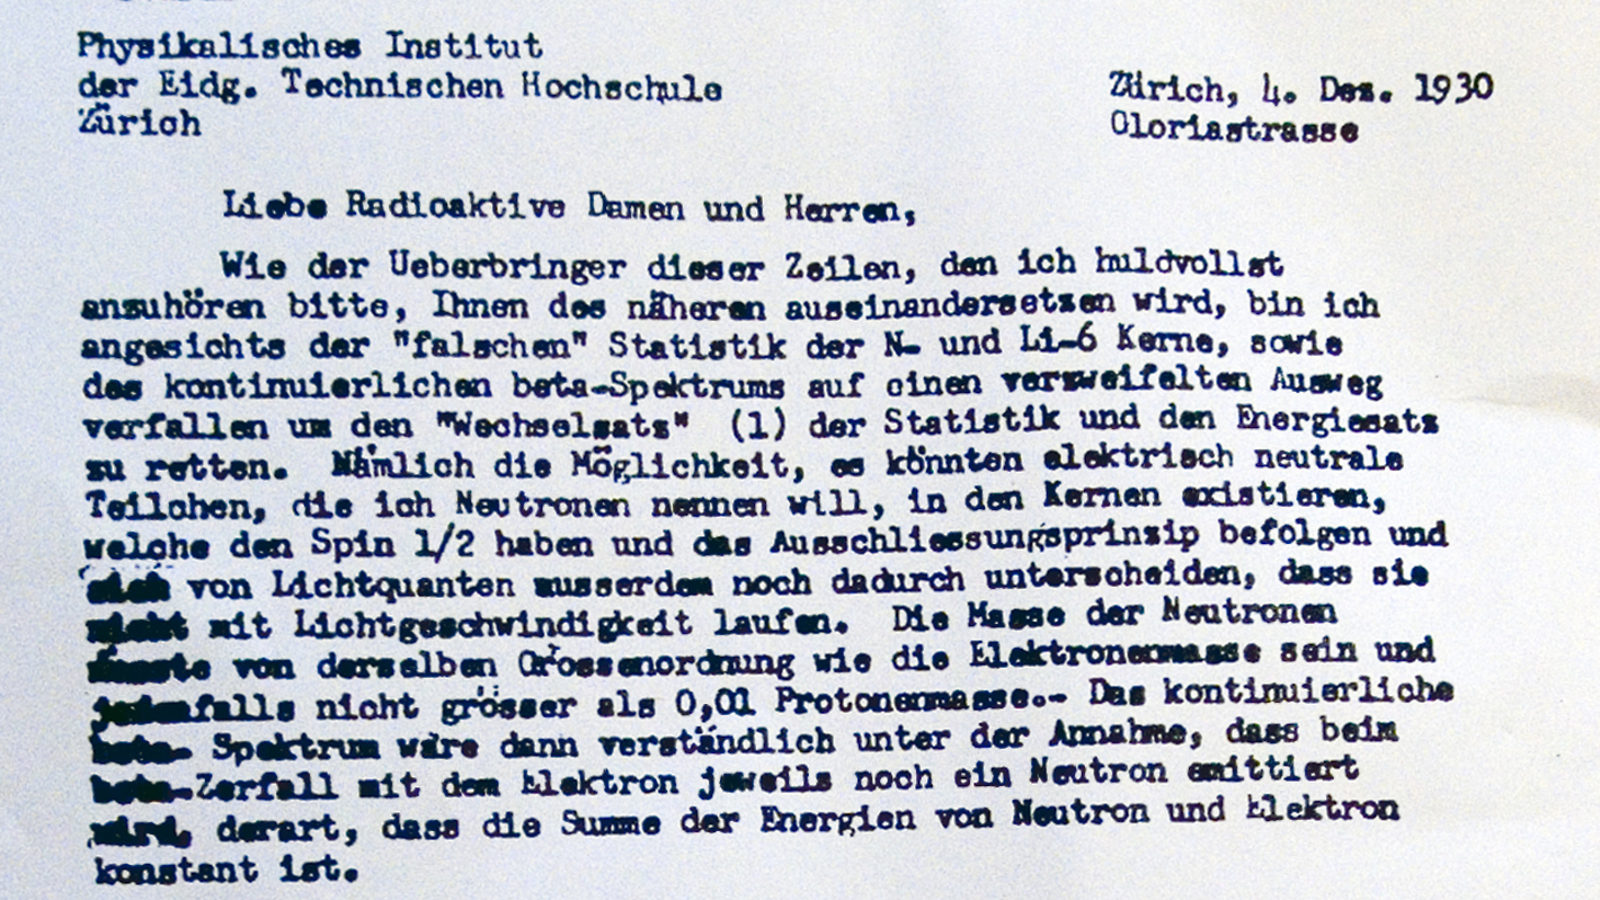
\includegraphics{theory/pauli_neutrino.jpg}
    \caption[Pauli's letter proposing the neutrino]{Pauli's open letter from December 1930, proposing the existence of the neutrino (he called it `neutron' at the time) to the community. Image credit: Pauli Letter Collection, CERN.}
    \labfig{pauli_letter}
\end{marginfigure}

Wolfgang Pauli reluctantly proposed the neutrino to explain the continuous $\beta$-spectrum of decaying uranium. When nuclear elements decay, they emit different particles. Their types of emission were dubbed $\alpha$-, $\beta$- and $\gamma$ radiation~\sidecite{Rutherford1899,Villard1900}; the first being helium-4 nuclei, the second electrons or protons, and lastly energetic photons. Contrary to $\alpha$- and $\gamma$-radiation, the spectrum of $\beta$-radiation turned out to be continuous, while one would expect discrete energy levels for the emitted particles.

In $\beta^-$-decay, the nucleus of an atom emits an electron when undergoing the nuclear transition $(A,Z)\rightarrow(A,Z+1) + e^-$. Here, $A$ is the mass number (the total number of nucleons in the atom), and $Z$ is the atomic number (the number of protons in the nucleus)---a neutron-proton conversion occurs, as is known nowadays. In this scenario, the decay is a two body problem, involving the nucleus and an electron. When converting a neutron into a proton, the resulting binding energy of the atom is lower, and this energy needs to be accounted for. Also, the positive charge gained by the nucleus during the transition must be equalized somewhere.

Therefore, the emitted electron carries the quantized energy lost to the atom due to its transition to the final state. As was already known at that time, this tight distribution of energy is fixed (by the difference in binding energy), so one would expect a narrow energy spectrum for the emitted electron, similar to $\alpha$- and $\gamma$-radiation. But the observed electron spectrum was continuous, hence the puzzlement of the community. Bohr proposed loosening the requirement of energy conservation---a suggestion Pauli was strongly opposed to\sidenote{He brought forth a though experiment of a closed box, within which $\beta$-decay happens. The weight of this box would change over time, a result he deemed paradoxical.}~\sidecite{Jensen2000}.

Pauli instead took refuge in what he considered a desperate solution, and suggested that the $\beta$-decay was in fact a three body problem, with a neutral particle carrying parts of the released energy~\sidecite{Bilenky2012}. This would explain the continuous electron spectrum. He also assumed that the hypothetical second particle interacted extremely rarely, which could explain why it had not yet been observed.

The next advancement in the understanding of the neutrino was due to Enrico Fermi in 1934. By then, the picture of the nucleus had been complemented by the neutron, discovered by James Chadwick two years earlier. Fermi developed the first theory of $\beta$-decay, analogous to the description of the emission of photons from excited nuclei~\cite{Fermi1934}. He assumed that the electron-neutrino pair is produced when a neutron within the nucleus transitions into a proton: $n \rightarrow p + e^- + \bar{\nu}$. The predictions from his theory were in fair agreement with observations, provided the neutrino mass was quite small~\cite{Fermi1934}.

\subsection{Neutrino Detections}
It took another 22 years until the neutrino was discovered experimentally. In the meantime, the nuclear bomb had been proposed, built, and used twice. The Savannah River Plant nuclear reactors were constructed as part of the effort to develop more fission bombs, producing plutonium and tritium. On a more pacifistic note, Reines and Cowan used the hypothesized flux of neutrinos from the reactors to first experimentally detect a neutrino~\cite{Reines1956} (with a confirmation in~\sidecite{Cowan1956}).

The experiment was based on the inverse beta decay, in which the predicted neutrino (in fact, an electron antineutrino) could react with a proton, converting it to a neutron and releasing a positron ($\bar{\nu_e} + p \rightarrow n + e^+$). The released positron would then annihilate with a free electron within the target material (for which they used $\text{H}_2\text{O} + \text{CdCl}_2$), releasing two \SI{511}{\kilo\eV} photons in the process, emitted in opposite directions due to conservation of momentum. These photons were then to be detected by a liquid scintillator surrounding the target. The neutron would diffuse through the target medium for a while until being captured by the cadmium, emitting a delayed photon signal (see Fig.~\ref{fig:neutrino_discovery}).

\begin{figure}[htb]
    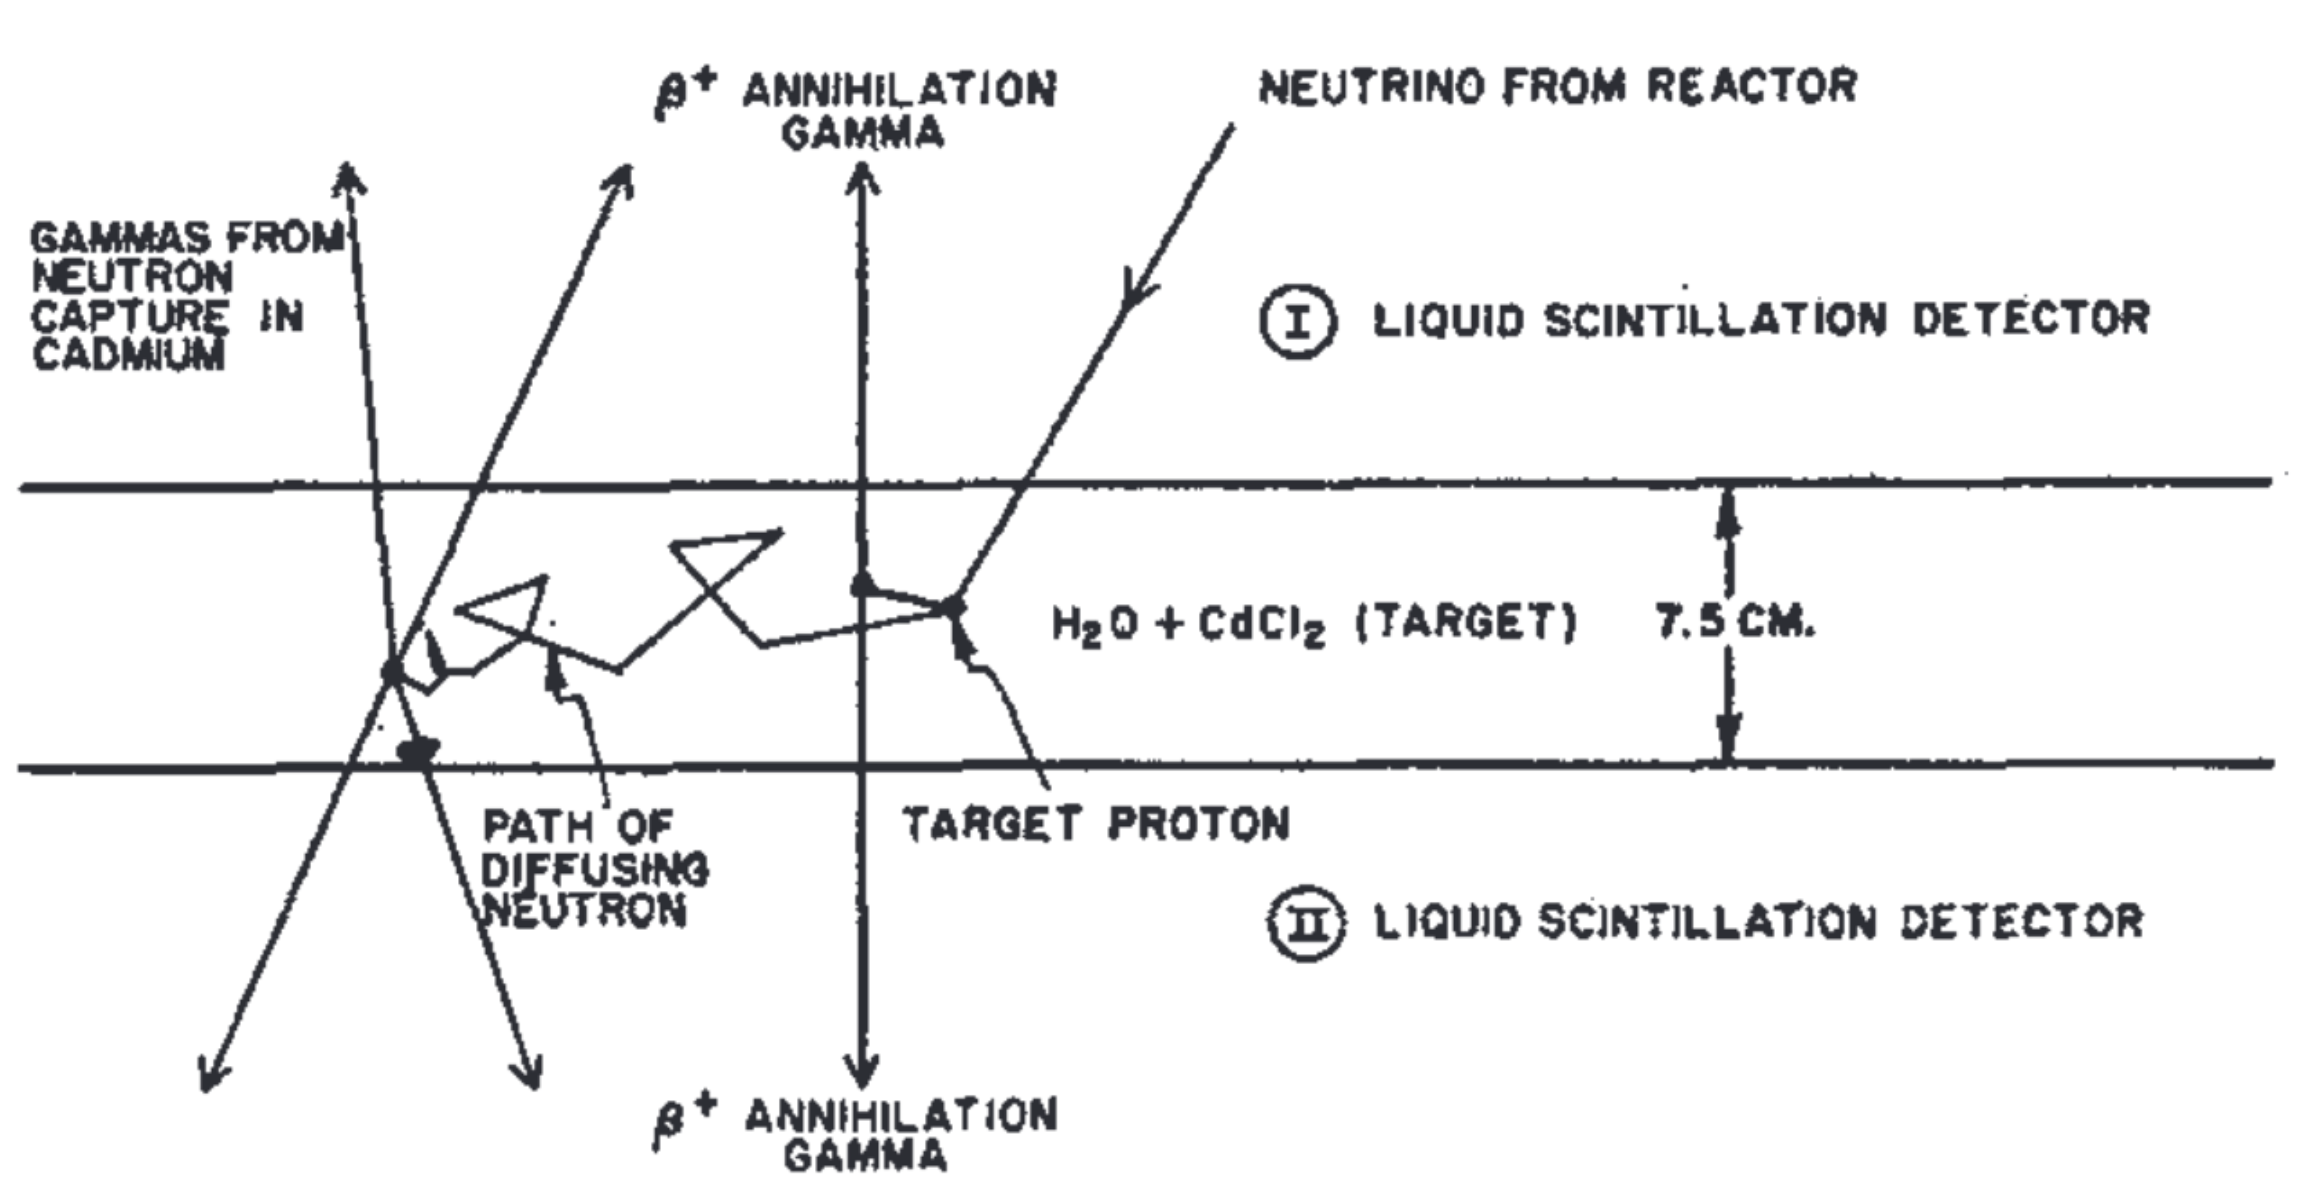
\includegraphics[width=0.8\textwidth]{theory/neutrino_discovery_principle.png}
    \caption[Neutrino discovery schematic]{Experimental setup for the discovery of the neutrino. From~\cite{Reines1956}.}
    \labfig{neutrino_discovery}
\end{figure}

The extremely low interaction rate, or in other words, the small interaction cross-section of the neutrino, required large amounts of target material and liquid scintillator to detect this reaction~\cite{Giunti2007}. Ultimately, thanks to the unique event signature described above, Reins and Cowan succeeded, reporting a neutrino detection rate of $2.88 \pm 0.22$ counts/hour~\cite{Reines1956}.

\subsection{Discovery of the Muon Neutrino}
Another important step was the discovery of the muon neutrino: At the Brookhaven National Lab in the US, muons and kaons from an accelerator were used to prove the existence of this neutrino flavor. Prior to the experiment, it had already been pointed out by Lee and Yang that the experimental failure to detect the decay $\mu \rightarrow e \gamma$ strongly hinted at the existence of a muon neutrino. This decay is only allowed if there is no difference between $\nu_e$ and $\nu_\mu$~\sidecite{Ekspong1993}.

The goal of the Brookhaven experiment~\sidecite{Danby1962} was to directly detect the muon neutrino by producing $\pi^+$ through bombarding a Beryllium target with \SI{15}{\giga\eV} protons. $\pi^+$ primarily decay to $\mu^+ + \nu_\mu$\sidenote{The channel $\pi^+ \rightarrow e^+ + \nu_e$ is strongly suppressed, see~\cite{Bilenky2012}.}. In a subsequent decay channel, almost all $\mu^+$ decay, only allowing the muon neutrinos to pass. These were directed towards a neutrino detector, consisting of aluminum plates located in a spark chamber. The neutrinos would interact with the aluminum nuclei and produce charged leptons. If there was no difference between $\nu_\mu$ and $\nu_e$, one would expect detecting $e^-$ and $\mu^-$ in virtually equal numbers.\ However, the experiment observed a significant number of muons (29) and detected only a few electrons (6), which could be attributed to background noise, thereby proving the existence of the muon neutrino~\cite{Danby1962}.

\subsection{The Solar Neutrino Problem}

\begin{marginfigure}
    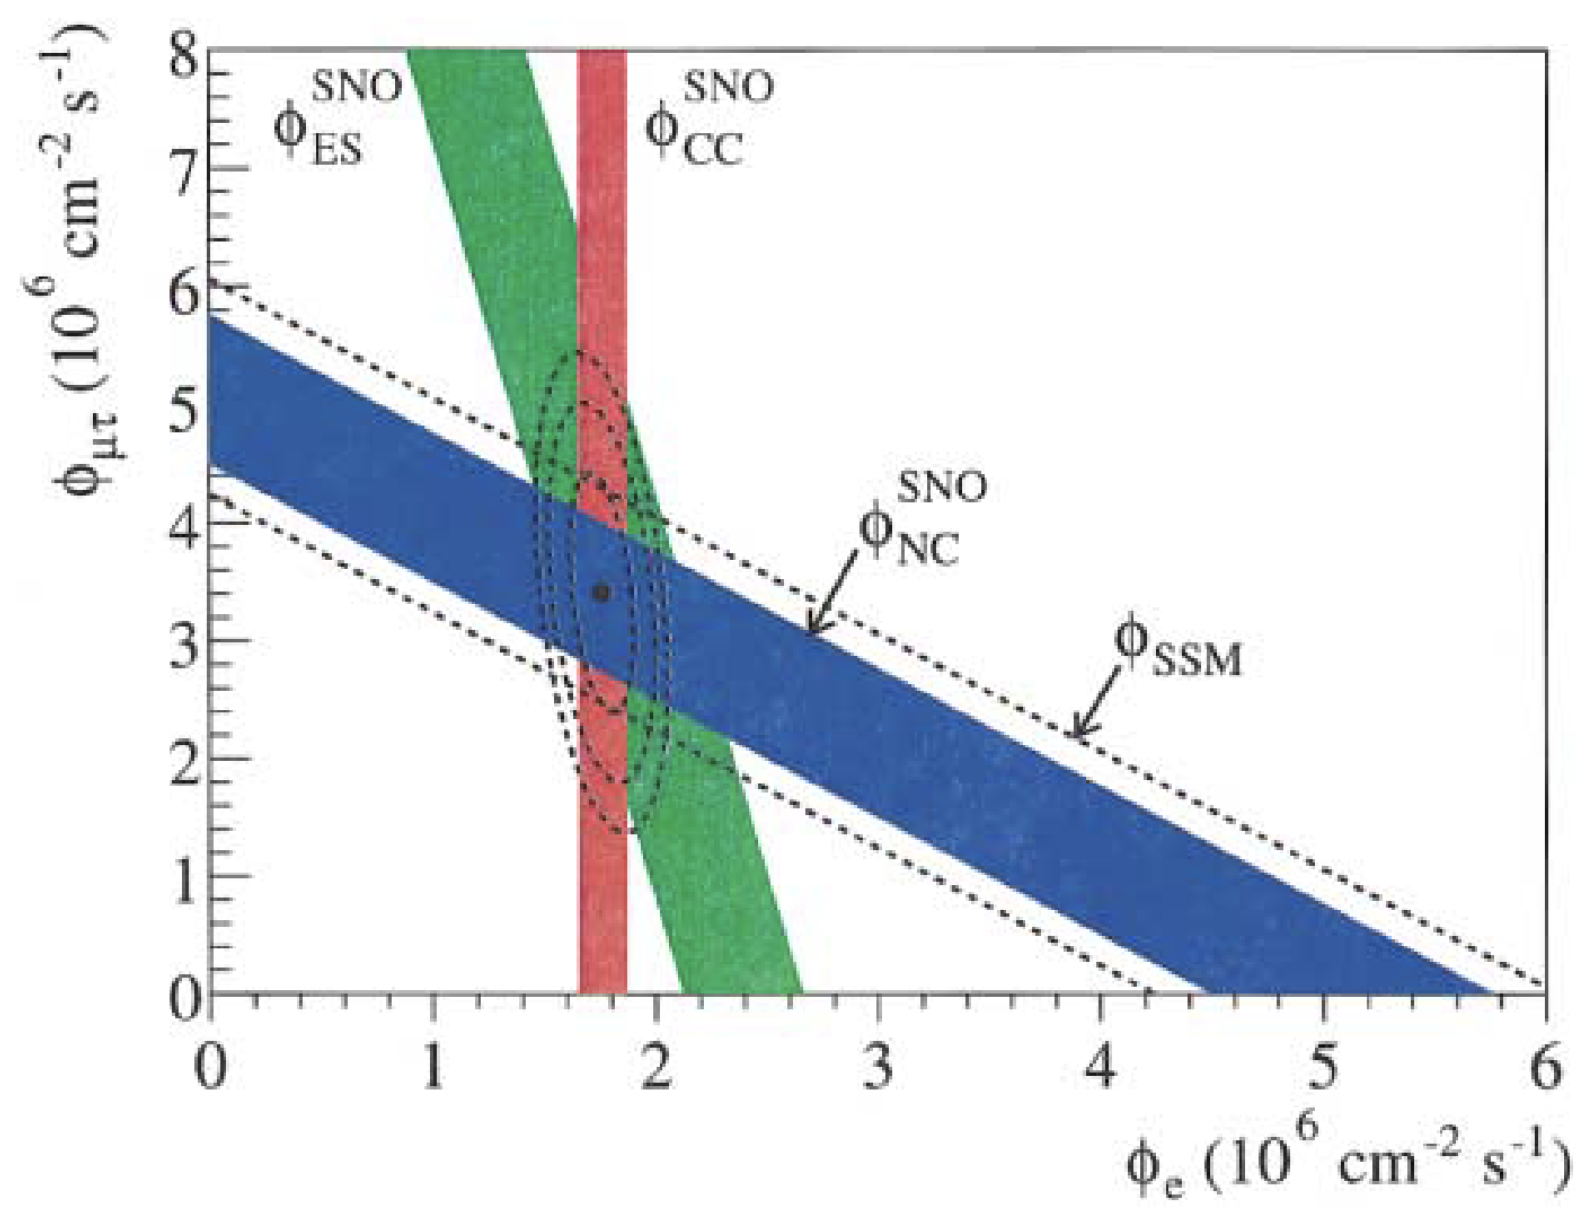
\includegraphics{theory/sno_flux.png}
    \caption[Solar neutrino flux measured by SNO]{The solar neutrino flux as measured by SNO\@. The x-axis shows the $\nu_e$ flux, while the y-axis shows the flux of solar $\nu_\mu$ and $\nu_\tau$. The intersection point shows the best-fit flux values for $\nu_e$ and $\nu_{\mu,\tau}$, with a resulting flavor ratio of $\sim1/3$ for all types. From~\cite{Ahmad2002}.}
    \labfig{sno_flux}
\end{marginfigure}

The neutrino was successfully detected. This, combined with the prediction that the process of nuclear fission within the sun should release neutrinos, triggered the hunt for solar neutrinos. The sun creates neutrinos both via the $pp$ chain and the CNO cycle, in both processes converting four protons and two electrons into a $^4\text{He}$ nucleus and two electron neutrinos: $4p + 2e^- \rightarrow  ~^4\text{He} + 2\nu_e + \SI{26.7}{\mega\eV}$. The energy is then released via photons or via neutrinos carrying kinetic energy~\cite{Giunti2007}.

Solar electron neutrinos were first detected in the 1960s in the Homestake experiment by Davis. He operated a tank located underground in the Homestake mine, filled with \SI{380}{\meter\cubed} of tetrachloroethene, which allowed antineutrino capture via $\nu_e +~ ^{37}\text{Cl} \rightarrow ~ ^{37}\text{Ar}^+ + e^-$. First results after 150 days of data taking resulted in an upper neutrino flux limit much lower than the theoretical expectations~\sidecite{Davis1968}. The experiment would run continuously from 1970 to 1994, detecting a neutrino flux that never exceeded \SI{50}{\percent} of the expected flux. The fact that the measured flux was consistently lower than the predicted one, despite various checks and improvements, became known as the solar neutrino problem~\sidecite{Bahcall1976}.

A solution to the solar neutrino was first proposed by Gribov and Pontecorvo in 1969~\sidecite{Gribov1969}: The missing electron neutrinos from the sun could have oscillated into neutrinos of a different flavor while traveling to Earth. This proposed neutrino oscillation was observed by the Sudbury Neutrino Observatory (SNO) in 2002; while evidence for the oscillation of atmospheric neutrinos had already been brought forth four years earlier by the Super-Kamiokande detector~\sidecite{Fukuda1998}. The SNO detector was sensitive to two types of interactions: One channel in which only $\nu_e$ could participate, and one open to neutrinos of all flavors. It was determined that the flux of solar $\nu_e$ was $\frac{1}{3}$ of the total neutrino flux (consisting of $\nu_e$, $\nu_\mu$ and $\nu_\tau$\sidenote{The existence of the tau neutrino had been confirmed one year earlier by the Direct Observation of the Nu Tau (DONUT) experiment~\cite{Kodama2001}.}). This result was in full agreement with theoretical predictions for the solar neutrinos flux, and directly showed that neutrinos do oscillate~\sidecite{Ahmad2002}.

These oscillations can be described by the $3\times3$ unitary transformation matrix known as the Pontecorvo-Maki-Nakagawa-Sakata (PMNS) matrix, that works analogous to the matrix describing the quark flavor mixing (Cabbibo-Kobayashi-Maskawa, or short CKM). The values of the matrix elements must be determined experimentally, as there is no underlying theory predicting them.

\subsection{Neutrino Mass}
By observing solar neutrino oscillations, the SNO experiment also established the fact that neutrinos have mass---contradicting the standard model of particle physics. Only massive particles allow oscillation between flavor eigenstates and mass eigenstates. It therefore does not make sense to ask for the mass of e.g.\ an electron neutrino, as this flavor eigenstate is a superposition of different mass states. One can speak of the effective electron neutrino mass, though; this is defined as

\begin{equation}\label{pmns}
    m_\nu = \sqrt{ \Sigma_i |U_{ei}|^2 m_i^2 },
\end{equation}

\begin{marginfigure}
    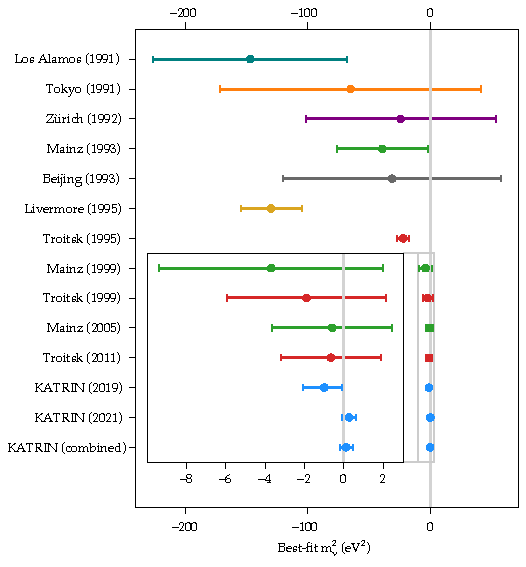
\includegraphics{theory/mass_history.pdf}
    \caption[Neutrino mass upper limit history]{The history of upper limits on the neutrino mass. From~\cite{Aker2022}.}
    \labfig{mass_history}
\end{marginfigure}

where $U$ is the PMNS matrix describing the neutrino state mixing, i.e.\ a collection of somewhat arbitrary numbers. If one could take individual mass measurements of the electron neutrino, one would measure the mass $m_i$ with probability $|U_{ei}|^2$.

Neutrino oscillations are only sensitive to the squared mass differences between the three mass states, as there is no zero point in Eq.~\ref{pmns}. One way to measure the average proper neutrino mass is the close inspection of the beta-decay\sidenote{See Section~\ref{neutrino_hypothesis}.} spectrum. The most recent in a long line of experiments to determine neutrino masses (see Fig.~\ref{fig:mass_history}) is the Karlsruhe Tritium Neutrino Experiment (KATRIN). It uses the beta decay of tritium. If the neutrino is massless, the energy spectrum of the emitted electron will extend up to the total energy of the decay (\SI{18.6}{\eV}). On the other hand, if the neutrino is non-zero, the electron energy will never exceed the energy of that neutrino mass. Note that in principle one could obtain all three neutrino masses from such an experiment if it weren't for current technological limitations. The latest upper limit from KATRIN on the neutrino mass is $m_\nu < \SI{0.8}{\eV}$ at the \SI{90}{\percent} confidence level~\sidecite{Aker2022}.


\subsection{Current Understanding}\label{neutrinos_current}
The Standard Model of particle physics knows three flavors of neutrinos, which are superposition of three mass states~\sidecite{Barger2012}. Their mass is small, but exists. Neutrinos have neither electromagnetic, nor color charge, but possess a weak hypercharge. This weak hypercharge lets them partake in weak interactions, which are mediated by exchanging $W$ or $Z$ bosons. Fig.~\ref{fig:neutrino_interactions} details some possible neutrino interaction channels, all constituting deep inelastic scattering with the quarks contained in nucleons. This is the dominant interaction mode for high-energy neutrinos with energies at or above several \unit{\giga\eV} in a medium.

\begin{figure}[htb]
    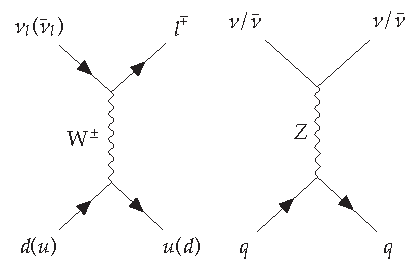
\includegraphics[width=0.5\textwidth]{theory/neutrino_interactions_feynman_short.pdf}
    \caption[Neutrino interactions]{Different neutrino interaction channels for deep inelastic scattering. Left: interaction of neutrinos (antineutrinos) with quarks by exchange of a $W^{\pm}$ boson, right interaction of neutrinos of all types by exchange of a $Z$ boson. The interaction on the right is called Neutral Current (NC) interaction, while the one on the left is dubbed Charged Current (CC) interaction.}
    \labfig{neutrino_interactions}
\end{figure}

Interactions that involve electromagnetically charged $W^-$ bosons are called Charged Current (CC) interactions, while those involving neutral $Z$ bosons are called Neutral Current (NC) interactions. For example, a neutron beta-decaying into a proton is a charged current interaction, as charge needs to be moved.

\begin{figure}[htb]
    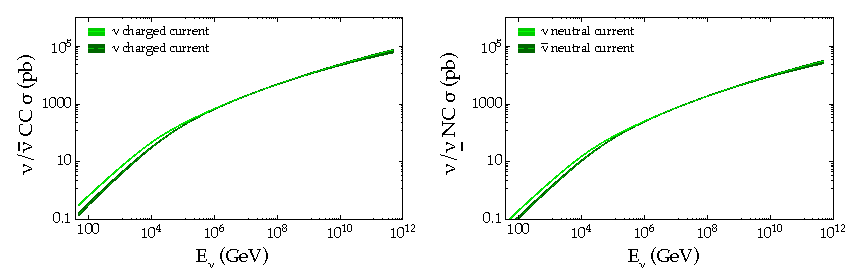
\includegraphics{theory/high_energy_nu_xsec.pdf}
    \caption[High-energy neutrino cross-section]{High-energy neutrino cross-section for interactions with matter equally composed of neutrons and protons. The unit on the y-axis are picobarn (\SI{e-40}{\m\squared}). The figure on the left shows charged-current interactions, while the one on the right displays neutral-current interactions, both for neutrinos and antineutrinos. Adapted from~\cite{CooperSarkar2011}.}
    \labfig{high_energy_nu_xsec}
\end{figure}

The cross-section for neutrinos with matter significantly increases with energy, as can be seen in Fig.~\ref{fig:high_energy_nu_xsec}. This is helpful for the detection of high-energy neutrinos, as this effect at least partially counterbalances the probable decrease in numbers of neutrinos produced in cosmic sources towards higher energies. On the other hand, neutrino detectors like IceCube are increasingly insensitive to neutrinos of the highest energies that sometimes have to traverse the Earth's core and get absorbed along the way.

For a better understanding of neutrino astronomy, it is beneficial to broadly divide the subject into two main categories, as the processes and instruments involved are fairly different: low-energy and high-energy neutrino astronomy. As high-energy neutrino astronomy is intertwined with cosmic-ray astrophysics is, a discussion of cosmic rays will be interspersed.

\section{Low-Energy Neutrino Astronomy}
Low-energy neutrinos, i.e.\ those carrying energies up to $\mathcal{O}(\unit{\mega\eV})$, are produced in stellar fusion processes and in supernovae. The primary stellar fusion process we can study is of course the sun.

\subsection{Stellar Neutrinos}
\begin{marginfigure}
    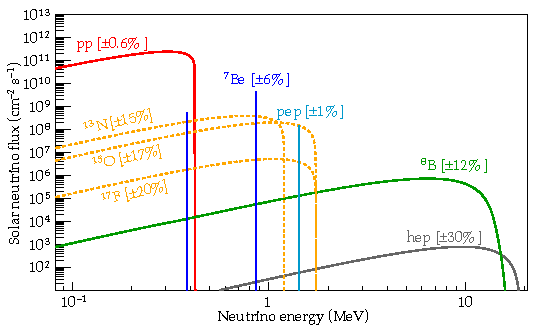
\includegraphics{theory/solar_neutrinos.pdf}
    \caption[Predicted solar neutrino flux]{Predicted solar neutrino flux. From~\cite{Agostini2018}.}
    \labfig{solar_neutrino_flux}
\end{marginfigure}

As briefly mentioned above, the solar neutrinos stem from two processes: The $pp$ chain and the CNO cycle. Within the $pp$ chain, neutrinos get produced by the proton-neutron conversion preceding the fusion of $p+n$ to $^2 \text{H}$. This conversion either happens via the $\beta^+$ decay $p \rightarrow n + e^+ + \nu_e$, resulting in a continuous neutrino spectrum (red curve in Fig.~\ref{fig:solar_neutrino_flux}), or via electron capture $e^- + p \rightarrow n + \nu_e$, which results in a line spectrum (leftmost blue line).

As one can see in Fig.~\ref{fig:solar_neutrino_flux}, the predicted solar neutrino spectrum is composed of different channels. Towards \unit{\mega\eV} energies, the solar neutrino flux is dominated by the decay of $^8\text{B}\rightarrow ~^8\text{Be} + e^+ + \nu_e$ (green curve) happening in one of the subsequent evolutions of the $pp$ chain. This particular process does not contribute much to the radiative energy output of the sun, but it was the responsible mechanism for the solar neutrino flux, of which $\frac{2}{3}$ were missing, constituting the aforementioned solar neutrino puzzle.

\begin{marginfigure}
    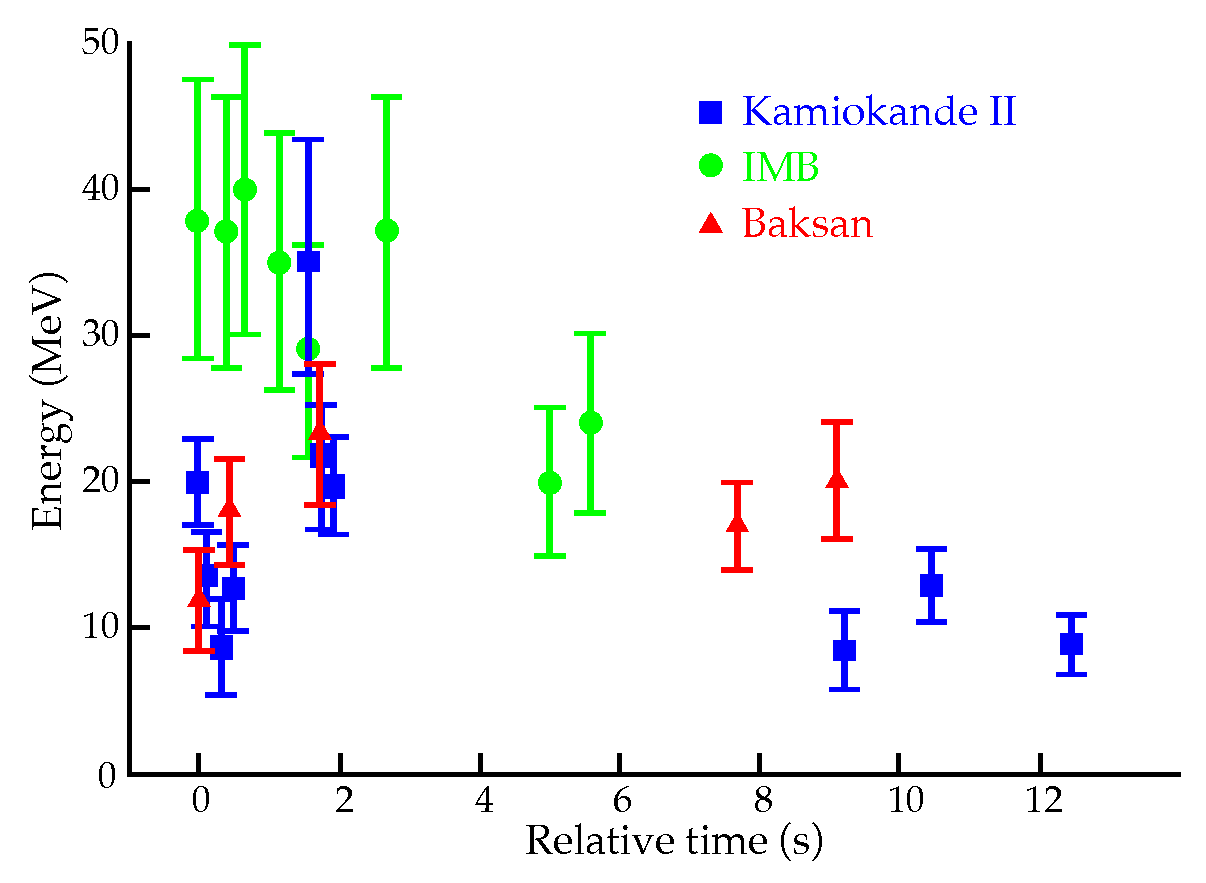
\includegraphics{theory/sn1987a_flux.pdf}
    \caption[Neutrinos from \emph{SN1987a}]{The neutrinos from \emph{SN1987a}, as measured by Kamiokande-II, IMB and BNO (Baksan). Figure\ adapted from~\cite{Grupen2005}.}
    \labfig{sn1987a_flux}
\end{marginfigure}

Fig.~\ref{fig:solar_neutrino_flux} also shows that the predicted flux cuts off around \SI{\sim10}{\mega\eV}, so only low-energy neutrinos are expected from the sun and similar stars.

\subsection{Supernovae}\label{sne}
Only with the first extragalactic neutrino source the era of neutrino astronomy truly began. This source was \emph{SN1987a}, an extremely close-by supernova in the Large Magellanic Cloud (LMC) that occurred in February 1987~\sidecite{Kunkel1987}.

Since Kepler's supernova almost 500 years ago\sidenote{It was a Type Ia supernova (see below) that occurred in 1604 in the Milky Way.}, \emph{SN1987a} was the first supernova observable by the naked eye alone, with an impressive brightness of $3-4$ mag due to its proximity~\sidecite{Spurio2018}.\ \emph{SN1987a} was the core-collapse of \emph{Sanduleak-69202}, a blue supergiant, resulting in a Type IIP supernova\sidenote{Though the rise instead of a plateau phase within its light curve gave it its own class, \emph{SN1987A}-likes~\cite{Arcavi2017}.}~\sidecite{Utrobin2021}. After the optical detection of the source the neutrino detectors Kamiokande-II, Irvine-Michigan-Brookhaven (IMB) and the Baksan Neutrino Observatory (BNO) found a burst of neutrinos predating the light from the supernova by 3 hours~\sidecite{Hirata1987,Bionta1987}, see also Fig.~\ref{fig:sn1987a_flux}.

In total, 25 neutrinos were detected by the three instruments (had IceCube already been operational in 1987, it should have detected \num{\sim13000} neutrinos~\sidecite{Halzen2017}). These rates were in agreement with theoretical models for core-collapse supernovae, assuming that \SI{99}{\percent} of the supernova energy is released in the form of neutrinos of all flavors.

Historically, supernovae are classified according to the presence of lines in their spectra. SNe of Type I lack hydrogen lines, in contrast to Type II SNe which do show hydrogen lines. Non-hydrogen SNe are further subdivided into SNe Ia that display silicon lines, SNe Ib that do not display silicon lines, but helium lines, and SNe Ic that have neither.

\subsubsection{SNe Ia}\label{sne_ia}
SNe Ia constitute a class sui generis. The underlying physical scenario for their explosion is often explained as a white dwarf accreting matter from a companion star (the so-called Single Degenerate (SD) scenario). The accretion eventually causes the star's mass to exceed the Chandrasekhar limit of $\sim1.4~M_\odot$. At this point the gravitational force overcomes the electron degeneracy pressure, and the star begins to burn carbon due to the increased pressure. Soon after that, a runaway thermonuclear reaction starts, and the white dwarf blows up violently~\sidecite{Iben1984}.

A second possible scenario that has recently gained traction is the Double Degenerate (DD) scenario. In this model, the SN Ia is the result of two gravitationally bound white dwarfs (a binary system) shedding gravitational energy in the form of gravitational waves and thereby slowly closing in on each other. Ultimately, they merge and cause the supernova explosion~\cite{Iben1984}.

In either scenario (see~\sidecite{Maoz2014} for a review), the luminosity of the resulting explosion can be standardized using the Philips relation~\sidecite{Phillips1993}. This makes SNe Ia standard candles, rendering them excellent instruments to measure cosmological distances. As they are mainly powered by the decay $^{56}\text{Ni}~\rightarrow~^{56}\text{Co}~\rightarrow~^{56}\text{Fe}$, they are expected to produce low-energy neutrinos, but not large quantities (when compared to core-collapse SNe, see next section)~\sidecite{Alsabti2017}.

\subsubsection{Core-Collapse Supernovae}\label{ccsne}

\begin{marginfigure}
    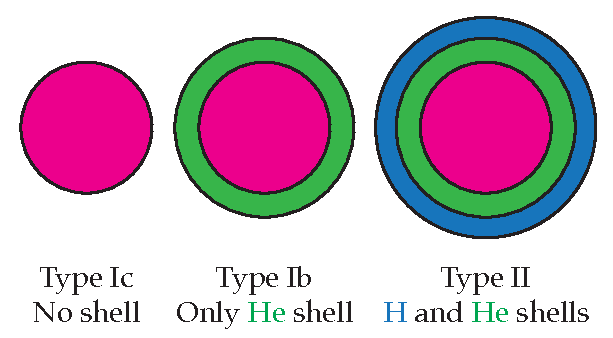
\includegraphics{theory/sn_shells.pdf}
    \caption[CCSN shells]{CCSN shells. The presence or absence of helium and hydrogen shells explains the differences in the respective spectra of CCSNe Type Ib, Ic and II. Because Ib and Ic Type SNe have lost parts of their outer shells, they are also referred to as Stripped-Envelope CCSNe. SNe IIb have almost lost their H shell, allowing them to quickly transform to a Type I SN.}
    \labfig{sn_shells}
\end{marginfigure}

In contrast to SNe Ia, all other types of SNe---no matter if they show hydrogen or not---are Core-Collapse Supernovae (CCSNe), resulting from the gravitational collapse of massive stars.

The spectral differences between SNe of Type Ib, Ic and II can be explained by the presence or absence of the two outermost shells: hydrogen and helium (see Fig.~\ref{fig:sn_shells}). If both shells are already far away from the star, the SN is of Type Ic (neither H nor He lines are present in the spectrum). If only the helium shell remains, the type is Ib, and if both shells are still present, the collapse will result in a Type II supernova.

Because Ib and Ic supernovae have partly or entirely shed their outermost shells, they are referred to as Stripped-Envelope (SE) SNe. SNe of Type IIb are also part of this class, as they initially display prominent hydrogen lines, which weaken over time until they disappear. This is most likely caused by the progenitor star having lost all but a thin shell of its hydrogen~\sidecite{Sravan2020}.

To complete the picture, some other subclasses of Type II SNe are motivated either by the presence of narrow lines in their spectrum (SNe IIn) or by a peculiar light curve evolution: SNe IIP show a plateau phase, while SNe IIL display a linear decay.

\subsubsection{Stellar Collapse}
Stars generate energy by first burning hydrogen. When a massive star has exhausted its hydrogen, fusion subsides and the gravitational pull compresses it further, until temperatures suitable for helium burning are reached. This process repeats for carbon, neon, oxygen and silicon. The silicon burning produces nickel, which decays to iron.

\begin{figure}[htb]
    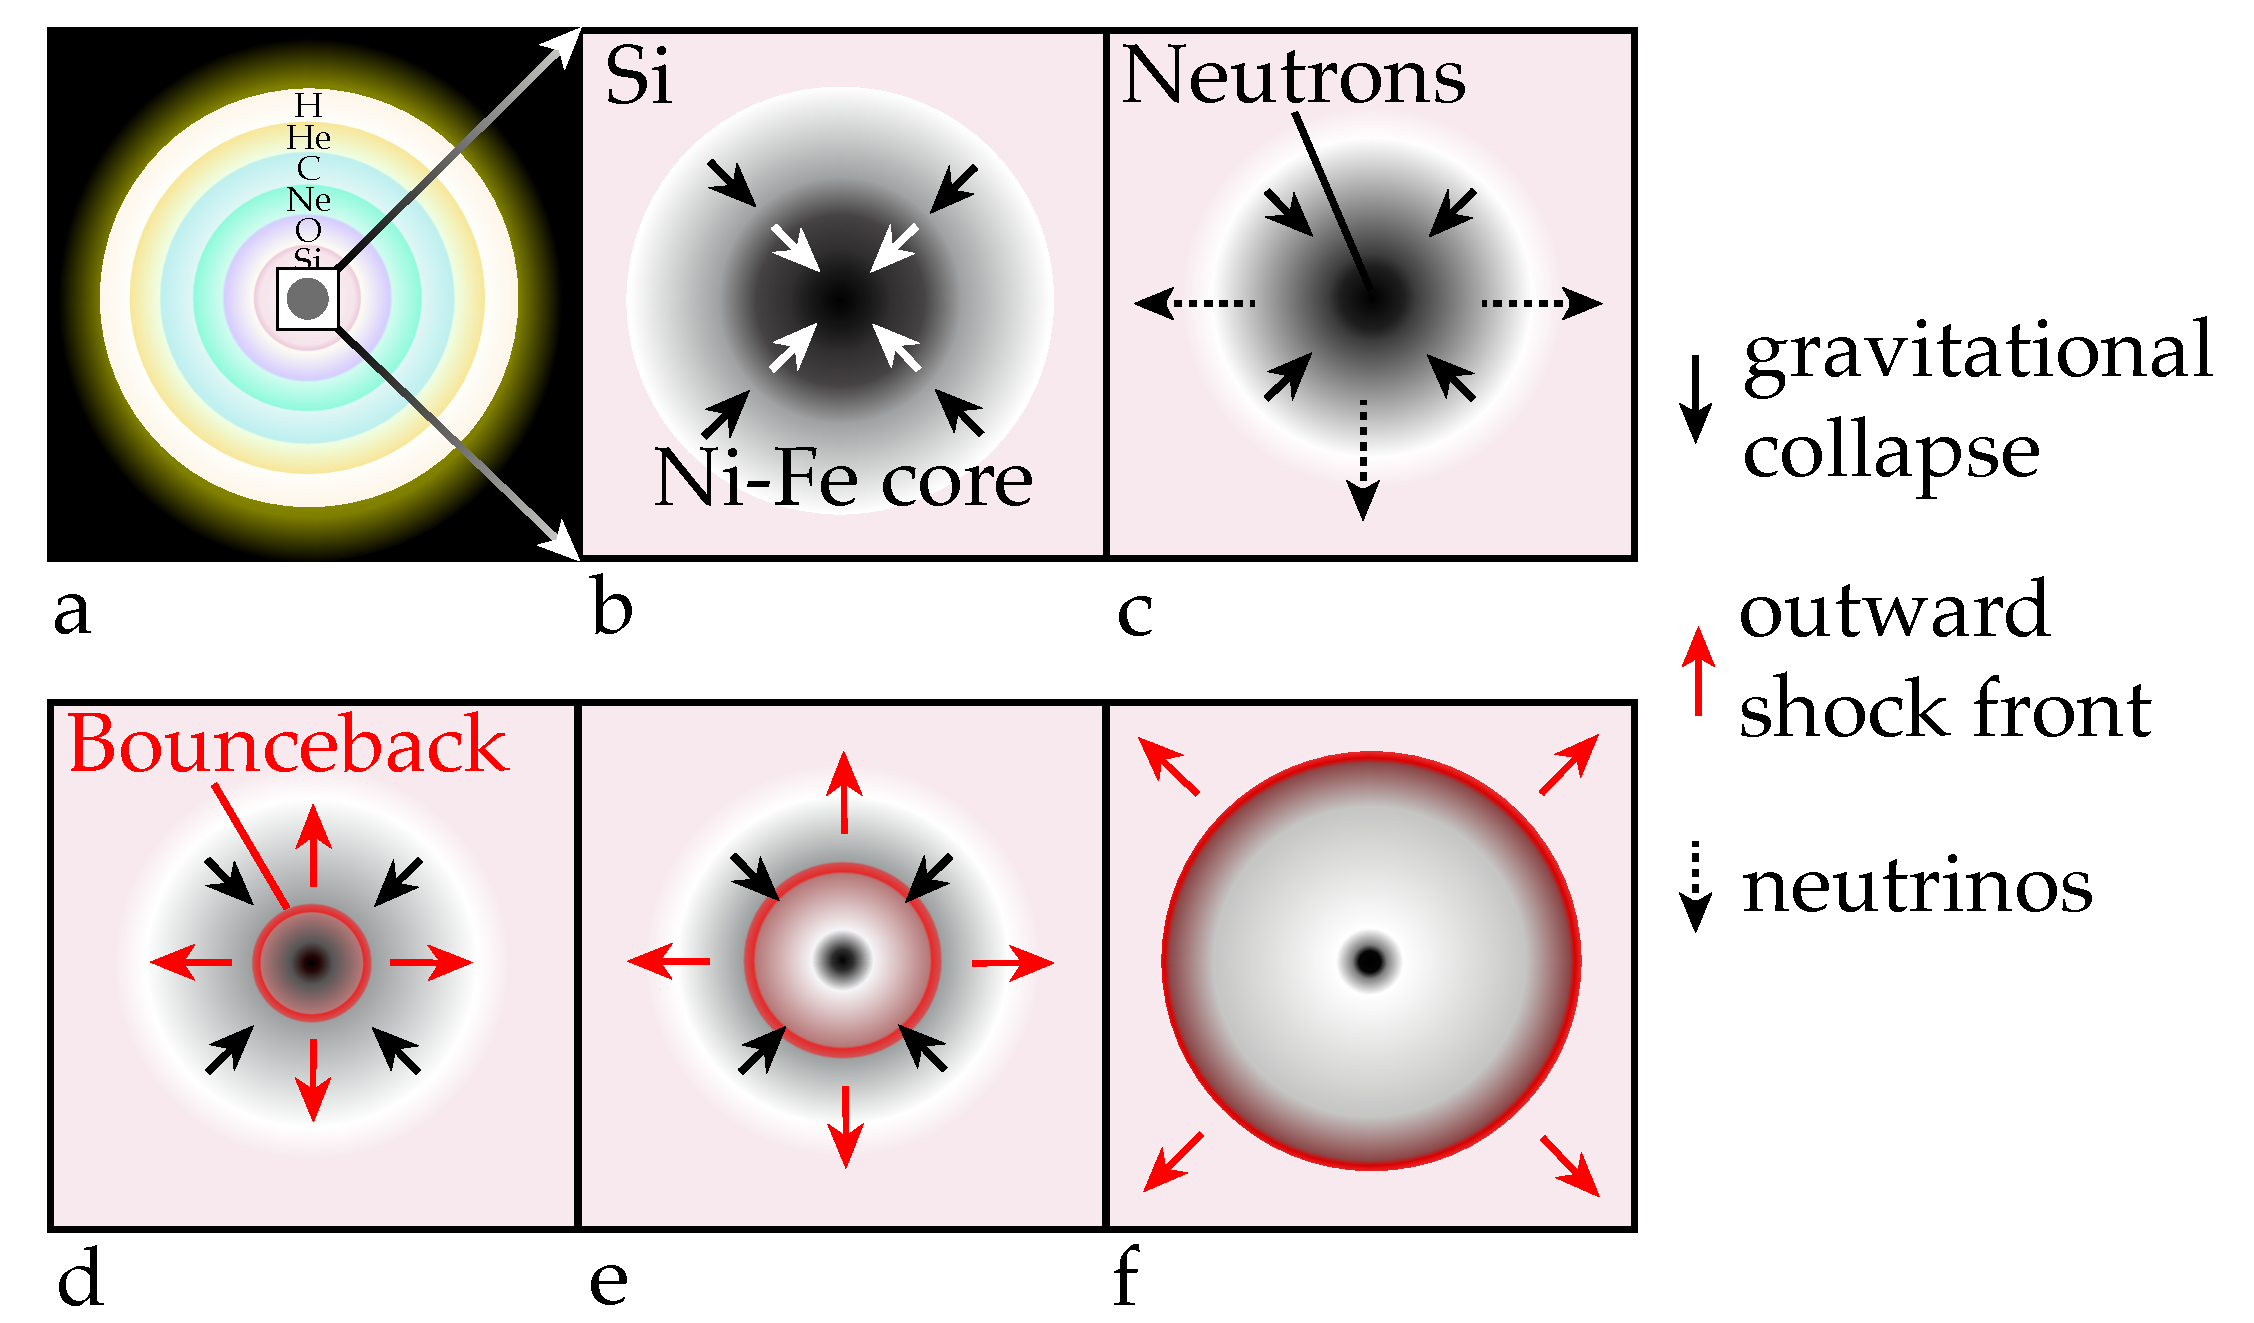
\includegraphics{theory/ccsn.pdf}
    \caption[Core-collapse supernova]{Schematic of a core-collapse supernova. Fusion stops in the core (b), causing it to collapse until neutron degeneracy prevents further collapse. A proto-neutron star forms in the center (c). The infalling material bounces back from the degeneracy border and forms a shock front (d). The stalling shock is reinvigorated by the intense flux of neutrinos from the proto-neutron star (e) and expands outwards (f). Adapted from \url{https://commons.wikimedia.org/wiki/File:Core_collapse_scenario.png} (which is most likely adapted from~\cite{Janka2012}).}
    \labfig{ccsn_schematic}
\end{figure}

A CCSN happens when a star with a mass between $8$ and $140~M_\odot$ has reached its final fusion stage, silicon burning, which ultimately produces iron. Iron has the highest binding energy of all elements, therefore fusing iron to heavier elements would release no energy, and the fusion chain stops. With the fusion subsided, the radiation pressure that so far prevented the star from collapsing in on itself suddenly vanishes. The infalling material compresses the core of the star within a second. As soon as the core becomes incompressible due to neutron degeneracy pressure described by the Pauli exclusion principle, the infalling material bounces back from the incompressible core and blows into the space around the former star. The remaining neutron star in the center either survives, or the infalling material eventually causes it to overcome neutrino degeneracy pressure and collapse into a black hole~\cite{Alsabti2017}.~

The more massive the star is, the higher the radiation pressure from fusion is. This radiation pressure is what drives the shedding of outer layers, so it is assumed that the most-stripped events, SNe Ic, result from a collapse of the most massive stars, followed by SNe Ib and lastly `regular' Type II supernovae, which have largely retained their outer shells.

In the centers of these core-collapse supernovae, neutron stars with masses of $1.5-2~M_\odot$ are created. These need to release large amounts of gravitational binding energy during the short moment of their creation. Because the environment at the center of the CCSN is dense and optically thick, photons are unable to escape: They immediately produce electron-positron pairs, which in turn are quickly absorbed by the surrounding matter.

Instead, \SI{99}{\percent} of the binding energy is carried away by neutrinos (see panels (e) and (f) in Fig.~\ref{fig:ccsn_schematic}). The energy radiated by the nascent neutron star via neutrinos typically amounts to \SI{\sim1.5e53}{\erg}, distributed equally over all three families, with a typical energy carried per neutrino of $\mathcal{O}(\SI{10}{\mega\eV})$~\sidecite{Lunardini2017}.

It has to be noted though that the exact mechanism the neutrinos play in the SN explosion is still insufficiently understood, as one has to rely on data from \emph{SN1987A} only, as well as numerical models. Eventually, a CCSN within our galaxy might come to the rescue~\sidecite{Janka2017}.

\section{Cosmic Rays}\label{cosmic_rays}

Now, there might also be more energetic neutrinos. But as these are thought to be produced during the same processes as cosmic rays, high-energy neutrinos are intricately linked to them. Therefore, one first needs a basic understanding of cosmic rays to understand high-energy neutrino production.

\begin{marginfigure}
    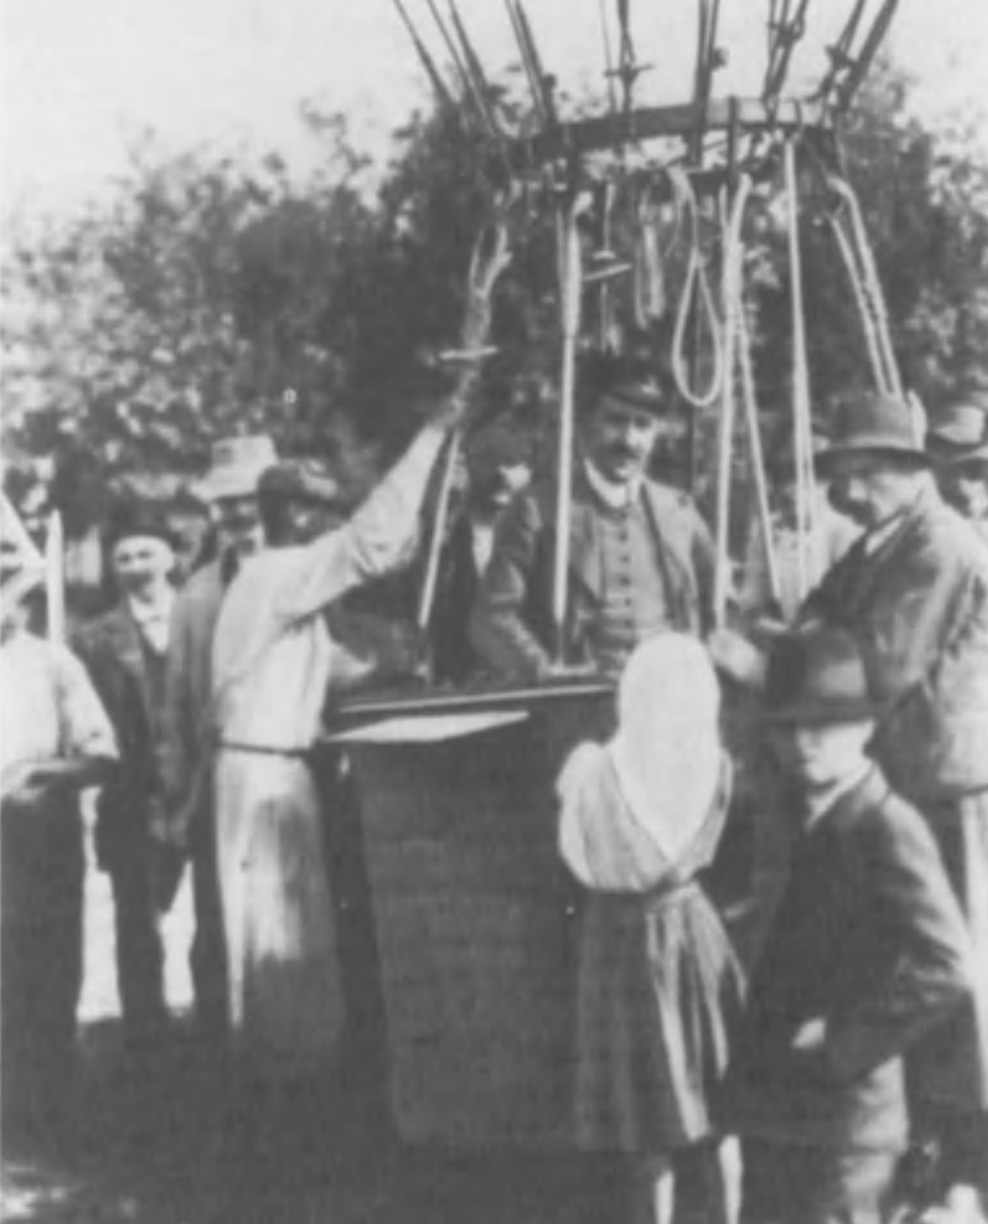
\includegraphics{theory/hess_balloon.png}
    \caption[Hess in his balloon]{Hess in his balloon after landing in Brandenburg, Germany in 1912, having just discovered cosmic rays. From~\cite{Steinmaurer1985}.}
    \labfig{hess_balloon}
\end{marginfigure}

\subsection{Discovery}

Cosmic rays were discovered in 1912 by Victor Hess. At the time, it had already been discovered that electroscopes---devices measuring electric charge and voltage---sometimes suddenly discharged. This was attributed to particles ionizing the air in the vessel, making it conductive and therefore allowing it to discharge. This was corroborated by the fact that reduced air pressure would slow the speed of the discharge. Another hint was that when shielding the isolated vessel, the ionization would decrease. The source of these ionizing particles was unknown, though.

Hess measured the flux of ionizing radiation with three electrometers during several balloon journeys. In total, he carried out 10 balloon ascents in the period of 1911--1913. The first ascent over \SI{5}{\km} in August 1912 marked the discovery of cosmic rays, when he registered a 16-fold increase in ionization measured by the electrometers at that height. Hess consequently concluded that the ionizing radiation must be of extra-terrestrial origin~\sidecite{Steinmaurer1985}.

\begin{marginfigure}
    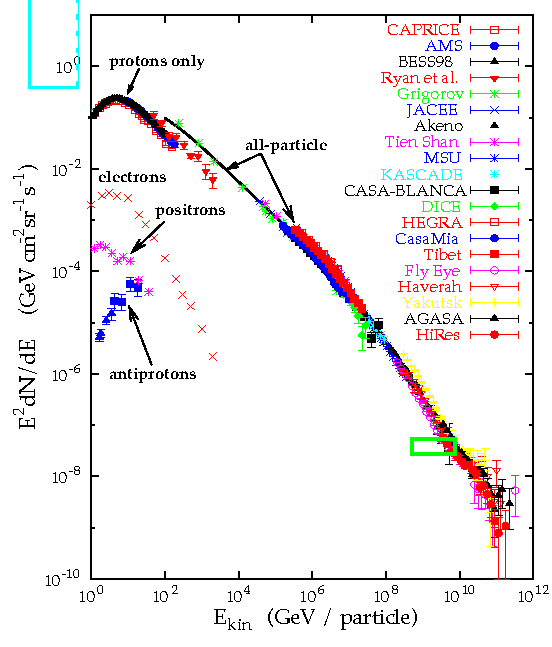
\includegraphics{theory/cr_spectrum.pdf}
    \caption[Cosmic ray spectrum]{Cosmic ray spectrum, as seen by a range of experiments. From~\cite{Hillas2006}.}
    \labfig{cr_spectrum}
\end{marginfigure}

\subsection{Composition and Energy Spectrum}

More than 100 years later, we know that this ionizing radiation consists of particles, spanning a broad range of energies. These particles are mostly protons, but all stable charged particles and nuclei with lifetimes of $\mathcal{O}(\SI{e6}{\year})$ can be found; most prominently protons, electrons, helium, but also e.g.\ carbon, oxygen and iron~\sidecite{Workman2022}.

As can be seen in Fig.~\ref{fig:cr_spectrum}, the cosmic ray spectrum spans a wide range of energies, from a few \unit{\mega\eV} up to \SI{e21}{\eV} (\unit{\zetta\eV}), with the high end of the energy spectrum constituting Ultra High-Energy Cosmic Rays (UHECR).

The UHECR part of the spectrum is shown in Fig.~\ref{fig:uhecr_spectrum}. It can be described by a series of power laws with different spectral indices, i.e. $E^{-\gamma}$, with $\gamma$ being the spectral index. The UHECR spectrum shows several interesting features, dubbed the Knee, the anatomically challenging Second Knee, and the Ankle. These are the points where the spectral index changes, and which are possibly associated with a transition to a new source class, e.g.\ from galactic to extragalactic sources around the ankle (see~\sidecite{Taylor2016}). This is still an active field of research~\cite{Workman2022}.

If high-energy neutrinos are produced in the processes responsible for the creation of cosmic rays (see below), the neutrinos stemming from cosmic rays with energies higher than the ankle should be mainly produced by extragalactic sources~\sidecite{Halzen2006}.

\begin{figure}[htb]
    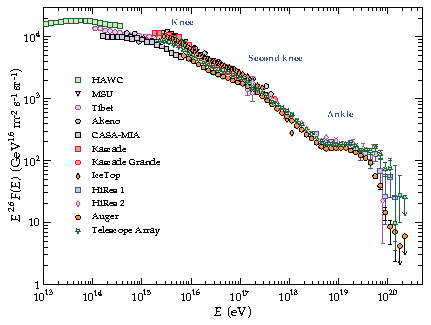
\includegraphics[width=0.8\textwidth]{theory/cr_uhecr_spectrum.pdf}
    \caption[UHECR spectrum]{Ultra high-energy cosmic ray spectrum. It shows energy per particle/nucleus vs.\ the flux (multiplied by $E^{2.6}$ to highlight the changes in spectral index). The data is from various air-shower experiments. From~\cite{Workman2022}.}
    \labfig{uhecr_spectrum}
\end{figure}

Identifying the sources of UHECR remains a challenge. As the cosmic ray particles are charged, they are deflected by magnetic fields encountered on their way to Earth, obscuring their origin. What is known though is that their extremely high energies necessitate extreme environments in which they can be produced.

In the 1980s, Hillas proposed the requirement that the efficient acceleration of a charged particle needs an accelerator that is able to confine the particle during acceleration: This means that the source needs to be larger than the particle's Larmor radius~\sidecite{Rieger2022}, i.e.~the radius of the circle a charged particle travels on given an external magnetic field. This introduces a bound on the possible sources for UHECR cosmic ray sources:

\begin{equation}
    E \leq 10^{20} Z \bigg(\frac{B}{\SI{10}{\micro\gauss}}\bigg) \bigg(\frac{R}{\SI{10}{\kilo\parsec}} \bigg)~\unit{\eV},
\end{equation}

\begin{marginfigure}
    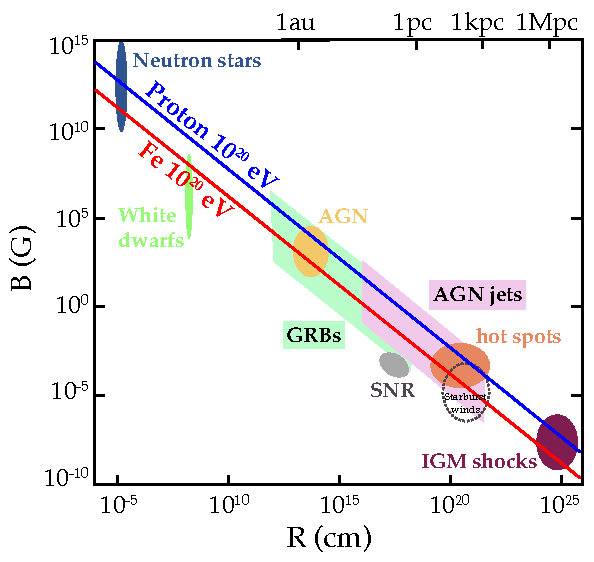
\includegraphics{theory/uhecr_hillas_criterion.pdf}
    \caption[Hillas source distribution]{Possible sources for \SI{e20}{\eV} cosmic rays, as a function of source radius $R$ and the magnetic field strength $B$ of the source. Adapted from~\cite{Rieger2022}, original `Hillas plot' in~\cite{Hillas1984}.}
    \labfig{uhecr_hillas_criterion}
\end{marginfigure}

where $Z$ is the cosmic ray particle charge number, $B$ is the magnetic field strength of the source, and $R$ is the characteristic source dimension~\cite{Rieger2022}. Sources that match this criterion for the production of UHECR protons and iron nuclei with an energy of \SI{e20}{\eV} are shown in Fig.~\ref{fig:uhecr_hillas_criterion}. As one can see, a variety of extreme environments are possible sources of UHECR. As some of these also hot candidates for the production of high-energy neutrinos, it is instructive to look at the mechanisms involved.

\subsection{Diffusive Shock Acceleration}\label{dsa}
There are several acceleration mechanisms for UHECR. The most important of these processes, Diffusive Shock Acceleration (DSA), was introduced in the late 1970s. DSA is thought to occur in the presence of shocks that are present e.g.\ in core-collapse supernovae\sidenote{See Section~\ref{sne}}. Such shocks are formed when matter, for example in the form of a plasma, is moving with supersonic speed through a surrounding medium.

To understand DSA, one has to differentiate between an upstream region in front of the moving shock front, and a downstream region behind the shock front.\sidenote{The majority of this section is owed to~\cite{Longair2011}.} Consider a shock front moving with a velocity $\vec{v_s}$ through a medium as seen in the observer's rest frame (red line in Fig.~\ref{fig:dsa}). If we switch to the rest frame of the shock front, it encounters the upstream medium as flowing towards it with speed $\vec{u_u}=-\vec{v_s}$. Downstream, behind the shock, the velocity of material $u_d$ will be lower: Mass conservation requires that $\rho_u u_u = \rho_d u_d$. In astrophysical shocks containing a fully ionized plasma, the compression ratio $R=\rho_d/\rho_u$ can be as high as 4~\sidecite{Longair2011}. Because $R=u_d/u_u$, the velocity of material downstream (behind the shock front) $u_d$ will then only be $1/4 u_u$.

Now consider some test particles upstream, ahead of the shock front rushing towards it. In the rest frame of the upstream gas their velocity distribution will be isotropic. Assume that the diffusion on both sides of the shock front is mediated via collisionless processes. This means that momentum and energy transfers between particles are mediated elastically by magnetic irregularities in the plasma (and Coulomb scattering can be neglected).

\begin{marginfigure}
    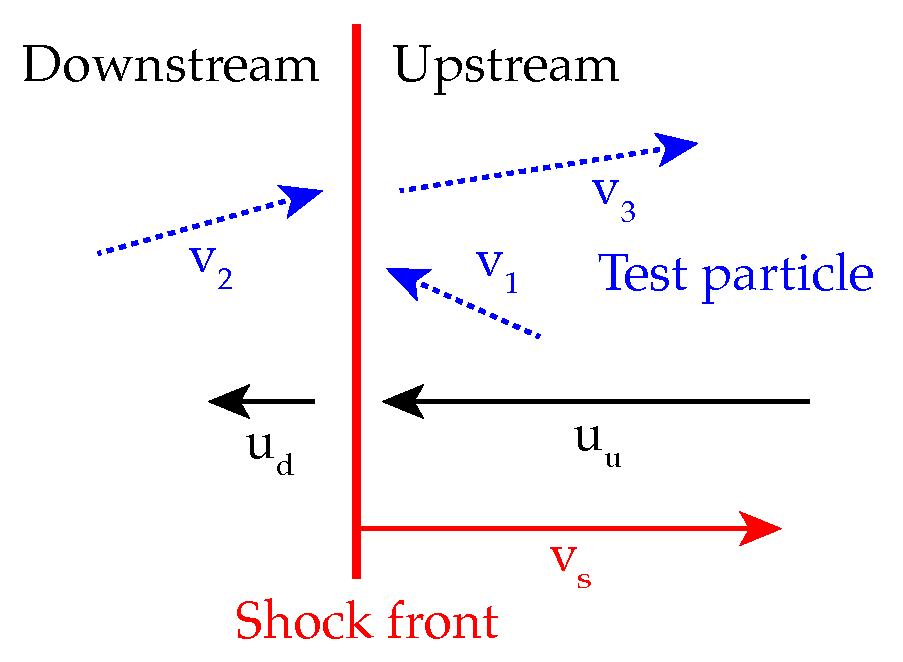
\includegraphics{theory/dsa.pdf}
    \caption[Diffusive shock acceleration]{Sketch illustrating diffusive shock acceleration. A shock front is moving with velocity $v_s$ with respect to an upstream medium. A test particle crosses the shock front twice, each time gaining energy. The length of the arrows are proportional to the velocity.}
    \labfig{dsa}
\end{marginfigure}

When a test particle with initial velocity $v_1$ (blue arrow in Fig.~\ref{fig:dsa}) eventually crosses the shock front to the downstream region, it will see a plasma rushing towards it with speed $w=|u_u-u_d| = (1-0.25)~u_u$, which equals 3/4 of the shock front velocity $v_s$.

In the downstream region, they will again be scattered collisionlessly, and receive a small net energy gain of $\big\langle\frac{\Delta E}{E}\big\rangle = \frac{2}{3}\frac{w}{c}$ (see below). This energy gain results in a higher velocity $v_2$. After some time, the particle might cross the shock front again, this time into the upstream region. From the now isotropized particle's frame, the upstream region will again rush in with $0.75~v_s$, and the process repeats, resulting in another gain in energy, and a higher $v_3$~\sidecite{Urosevic2019}, with an average round-trip energy gain of $\big\langle\frac{\Delta E}{E}\big\rangle = \frac{4}{3}\frac{w}{c}$

We still need to motivate the net energy gain per crossing of $\big\langle\frac{\Delta E}{E}\big\rangle = \frac{2}{3}\frac{w}{c}$. This can be explained as follows: First, one needs to switch to the test particle frame, i.e.\ perform a Lorentz transformation. The energy of the test particle will be:

\begin{marginfigure}
    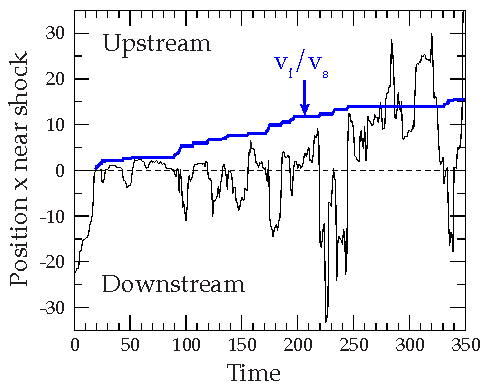
\includegraphics{theory/dsa_mc.pdf}
    \caption[DSA Monte Carlo]{Monte Carlo simulation of a test particle near the shock front. The particle position wildly varies (solid line), but its velocity $v_i$ (dotted line) increases each time it crosses the shock front at $x=0$. Adapted from~\cite{Baring1997}}
    \labfig{dsa_mc}
\end{marginfigure}

\begin{equation}
    E' = \gamma_{w}(E+p_x w),
\end{equation}

where x is the coordinate perpendicular to the shock. The shock is non-relativistic ($w<<c$ and $\gamma_w\approx1$), but the test particles are, so $E\approx pc$ and $p_x \approx E/c \cos(\theta)$. From this it follows that

\begin{equation}
    \Delta E = E' - E = E+\frac{E}{c}w\cos{\theta}-E = pw\cos{\theta}
\end{equation}

and

\begin{equation}
    \frac{\Delta E}{E} = \frac{p}{w}\cos{\theta} = \frac{w}{c}\cos{\theta}.
    \label{eqn:delta_e_over_e}
\end{equation}

The probability of the test particle angle $\theta$ to lie between $\theta$ and $\theta + \text{d}\theta$ is proportional to $\sin{\theta}\text{d}\theta$, and the test particle approach rate is proportional to $v_x = \frac{p_x}{m} = \frac{E/c\cos{\theta}}{E/c^2} = c \cos{\theta}$. The probability of the test particle crossing the shock front is therefore proportional to $\sin{\theta} \cos{\theta} \text{d}\theta$. The integral from 0 to $\frac{\pi}{2}$ is 0.5, so we need to multiply by 2 to normalize the cumulative probability to 1:

\begin{equation}
    p(\theta) = 2\sin{\theta}\cos{\theta} \text{d}\theta
\end{equation}

By integrating $p(\theta)$ and using Eq.~\ref{eqn:delta_e_over_e}, we can calculate the average energy gain of each shock crossing:

\begin{equation}
    \bigg\langle \frac{\Delta E}{E} \bigg\rangle = \int_0^{\pi/2} \frac{\Delta E}{E} p(\theta) = \frac{w}{c} \int_0^{\pi/2} 2 \sin{\theta} \cos^2{\theta}  \text{d}\theta = \frac{2}{3}\frac{w}{c}
\end{equation}

After another crossing, the test particle will gain another average energy increase of $\frac{2}{3}\frac{w}{c}$, resulting in an average energy gain of $\frac{4}{3}\frac{w}{c}$ per round trip~\cite{Longair2011}.

During each crossing, a particle with initial energy $E_0$ will gain an energy fraction $\beta$, resulting in energy $E=\beta E_0$. If $P$ denotes the probability that a particle stays within the accelerating region, the number of particles after $k$ crossings can be written as $N=N_0 P^k $, and they will have energies $E=E_0\beta^k$.

If one solves both equations for $k$ and sets them equal, one obtains
\begin{equation}
    \frac{\ln (N/N_0)}{\ln (E/E_0)} = \frac{\ln P}{\ln \beta}.
\end{equation}

By rearranging we get

\begin{equation}
    \frac{N}{N_0} = \bigg(\frac{E}{E_0}\bigg)^{\ln P / \ln \beta}
\end{equation}

To obtain the differential energy spectrum, we differentiate with respect to $E$ and get

\begin{equation}
    \label{eqn:diff_e_spec}
    N(E)~\text{d} E = C\times E^{(\ln P/\ln\beta)-1}~\text{d} E
\end{equation}

The result is a power law with index $\frac{\ln P}{\ln \beta}$, which is indeed what was already stipulated by experimental data.

We already know that $\big\langle\frac{\Delta E}{E}\big\rangle = \frac{4}{3}\frac{w}{c}$. With this, $\beta = \frac{E}{E_0} = 1 + \frac{4}{3}\frac{w}{c}$. What is missing is an expression for $P$. To obtain this, we need to estimate the rate at which particles drop out of the system or are `swept away'. As argued by~\cite{Longair2011} (and originally presented by~\sidecite{Bell1978}), the average number of particles crossing the shock is $\frac{1}{4} n c$, with $n$ being the particle number density. This is true in both directions up- and downstream. The difference though is that downstream particles are `advected' away from the shock further downstream and out of the system, as they are isotropic in that frame. The dropout rate is $n w=\frac{1}{4}nv_s$. From this it follows that the fraction of particles lost (per unit time) is $\frac{1}{4} n v_s/\frac{1}{4}nc = v_s/c$. The survival probability $P$ is thus $P=(1-v_s/c)$.

With that, we can compute
\begin{equation}
    \ln P = \ln ( 1-\frac{v_s}{c}) \simeq -\frac{v_s}{c}
\end{equation}
and
\begin{equation}
    \ln \beta = \ln(1+\frac{4}{3}\frac{w}{c}) \simeq \frac{4}{3}\frac{w}{c} = \frac{v_s}{c}.
\end{equation}
This gives us $\frac{\ln P}{\ln \beta} \simeq -1$. Inserting this into Eq.~\ref{eqn:diff_e_spec} yields
\begin{equation}
    N(E)~\text{d} E \propto E^{-2}~\text{d} E.
\end{equation}

Therefore, the resulting differential energy spectrum has a spectral index of 2. This somewhat differs from the experimentally found spectral index of 2.7 up to the knee. This can be explained by the fact there are several assumptions at play here: The shock is assumed to be non-relativistic, in an ideal gas and constant escape probability. Inefficiencies in the shock, and the inclusion of shock-amplified magnetic fields can both harden the spectral index~\cite{Spurio2018}.

\subsection{Interaction and Neutrino Production}\label{cr_interactions}
As discussed above, the observed cosmic ray spectrum is readily explained by astrophysical shocks, as these account for the power-law structure of the energy distribution.

The particles accelerated within shocks might now interact with either hadrons and photons in their vicinity or on their way to Earth. For simplicity, this section focuses on the interaction of cosmic ray protons, but it applies to heavier nuclei as well.

\begin{description}
    \item[$pp$ interactions] When cosmic ray protons encounter gas, either at the source location or while crossing the universe, they can interact with this gas, here assumed to consist of protons only for simplicity. The resulting $pp$ interactions produce lots of unstable hadrons, which decay. Those decays are dominated by pion production. Ignoring all secondary hadrons $X$ (which can also decay via pions), possible decay channels of these pions are:

          \begin{eqnarray}
              \pi^\pm + X &\contour{black}{$\rightarrow$}& \mu^\pm + \nu_\mu (\bar{\nu}_\mu)~~~ \contour{black}{$\rightarrow$} ~~~ e^\pm + \nu_e(\bar{\nu}_e) + \bar{\nu}_\mu(\nu_\mu)\\
              \pi^0 + X &\contour{black}{$\rightarrow$}& 2\gamma
          \end{eqnarray}
          As can be seen, $\pi^\pm$ decay into muons and a muon (anti-)neutrino. Those muons will decay into electrons (positrons), electron (anti-)neutrinos and muon (anti-)neutrinos. The decay of the neutral $\pi^0$ does not generate neutrinos. For pion decays, an average neutrino flavor content of $\nu_e$:$\nu_\mu$:$\nu_\tau = 1:2:0$ is expected. Neutrino oscillation on the way to Earth washes out this initial difference, with an expected flavor content of $1:1:1$~\cite{Workman2022}.


          The energy of the pion decay products is expected to trace the initial proton energy spectrum. If the proton interaction rate is fairly independent of their energy, they will then lose a fraction of their energy. This energy will then be converted into the production of pions, and subsequently muons. With this, the resulting neutrino spectrum is expected to have a similar shape as the initial cosmic ray spectrum.\todo{source or rephrase}


    \item[$p\gamma$ interactions]
          Cosmic ray protons can also interact with radiation fields. The cross-section for these interactions is large near the $\Delta^+$ resonance. The dominant $\Delta^+$ decay modes again contain pions:
          \begin{eqnarray}
              \Delta^+ ~~ &\contour{black}{$\rightarrow$}& n + \pi^+ \\
              \Delta^+ ~~ &\contour{black}{$\rightarrow$}& p + \pi^0
          \end{eqnarray}
          The pions will again decay according to the channels already discussed for $pp$ interactions. The secondary neutrons might decay via beta decay, and produce electron antineutrinos. Here, the shape of the neutrino spectrum not only depends on the proton spectrum, but also the photon spectrum. Therefore, it is not expected to trace the shape of the initial cosmic-ray spectrum~\sidecite{Fiorillo2021}.
\end{description}


\section{High-Energy Neutrino Astronomy}\label{he_neutrino_astronomy}

As shown above, high-energy cosmic ray particles can produce high-energy neutrinos in $pp$- or $p\gamma$-interactions. These high-energy neutrinos have energies in the \unit{\mega\eV} range and above. But what are possible source classes for these? There will be some overlap with the low-energy neutrino events, as some of those---like e.g. supernovae---are also probable sources of high-energy neutrinos.

\subsection{Interacting Supernovae}\label{interacting_sne}
As already detailed in Section~\ref{sne}, core-collapse supernovae are thought to produce copious amounts of \unit{\mega\eV}-neutrinos. Interestingly, certain types of CCSNe are thought not only to produce such comparably low-energy neutrinos, but also \unit{\giga\eV} to \unit{\tera\eV} neutrinos. Optical observations have stipulated that supernova progenitors often violently eject material into the circumstellar region in the years to centuries prior to their explosion~\sidecite{Ofek2014}. When the supernova happens, ejecta are driven into this circumstellar material (CSM).

SNe of Type IIn are a subclass first stipulated by Schlegel~\sidecite{Schlegel1990}: The Balmer emission features of early IIn spectra, most prominently the $H_\alpha$ region, show narrow lines on top of a broad component~\sidecite{Taddia2013}. The broad component is caused by the supernova itself, but the narrow lines result from interaction of the SN blast-wave with the CSM. This process photo-ionizes the CSM, which results in narrow hydrogen lines.

Such a system might be promising for the production of high-energy neutrinos, as highlighted in~\sidecite{Kurahashi2022}. When the SN ejecta---expanding with velocities of \SIrange{3000}{10000}{\km\per\s}---hit the CSM, a shock wave starts to propagate through it. Particle acceleration within the shock is predicted to happen at the moment of shock breakout. This is the time when the optical depths of the shock drops below $\approx c/v$, with $v$ being the shock velocity. As soon as the radiation can escape, the shock is no longer radiation-mediated, and protons can be accelerated to high energies~\sidecite{Waxman2017}. This emission seizes after the shock decelerates or reaches the outer edge of the CSM.

These accelerated protons are expected to generate high-energy neutrinos, either by $pp$ or $p\gamma$ interactions (see Section~\ref{cr_interactions}). The resulting neutrinos are expected to range from \unit{\giga\eV} to hundreds of \unit{\tera\eV}, reaching their maximum flux shortly after shock breakout~\sidecite{Petropoulou2017,Murase2018}.

The signature of such an event is expected to be a high-energy neutrino detected close to the optical peak of a supernova that shows signs of CSM interaction, i.e.\ has narrow lines in the optical spectrum.

\subsection{Gamma-ray Bursts}\label{grb}
Gamma-ray bursts (GRBs) were discovered by accident by the \textit{Vela} satellites designed to monitor nuclear detonations as part of a partial test ban treaty between the US and the USSR in the 1960s. 16 bursts of high-energy photon events recorded by those satellites were published in 1973. This kicked off a flurry of research, as a terrestrial or solar origin of these gamma-ray bursts could be excluded~\sidecite{Klebesadel1973}.\todo{maybe remove the cliffhanger: why could this be excluded?}

The gamma-ray light curves of these very bright and brief events last from a few milliseconds to tens, sometimes hundreds of seconds~\sidecite{Vedrenne2009}. As more and more GRBs were registered, a bimodal population was recognized: Short GRBs (sGRBs), with an average duration of $\SI{\sim0.3}{\s}$, and long GRBs (lGRBs) that typically last \SIrange{10}{20}{\s}.

The most prevalent interpretation of these two populations is that short GRBs stem from the merger of two compact objects, e.g.~neutron stars. This was hypothesized for a long time, and found spectacular confirmation with the association of the short gamma-ray burst GRB170817A detected \SI{1.7}{\s} after a gravitational wave signal was detected from the same region (GW170817), most likely stemming from the merger of two neutron stars~\sidecite{Abbott2017}.

Meanwhile, long GRBs are hypothesized to be the signatures of jets launched by CCSNe~\sidecite{Galama1998}. The existence of such jets has been proposed already in the 1970s; see e.g.~\sidecite{Leblanc1970}. If these jets manage to punch through the stellar envelope and the surrounding CSM, one can detect them as long GRBs. Virtually all CCSNe that could be associated with a prior long GRB are Broad-Line Ic (Ic-BL)~\sidecite{Pian2017}, i.e.\ collapses of highly stripped, massive stars with large ejecta velocities.

Both short and long GRBs have been proposed as potential sources of high-energy neutrinos. For short GRBs, neutrinos are only attributable to a source if a GRB afterglow is detected, i.e.\ longer lasting X-ray, optical and radio emission~\sidecite{Waxman1997}. The event signature as accessible by IceCube and ZTF (see next two chapters) would be a prompt high-energy neutrino coincident with the gamma-ray signal, accompanied by optical emission quickly fading over the subsequent days.

\begin{figure*}[htb]
    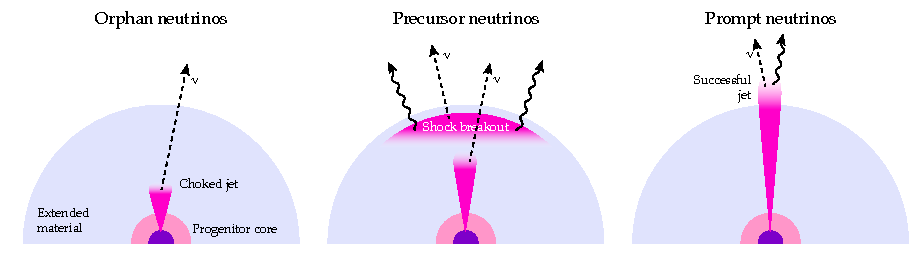
\includegraphics[width=1.4\textwidth]{theory/grb_model.pdf}
    \caption[High-energy neutrinos from GRBs]{Concordance scenario for neutrinos from failed, semi-failed and successful jets launched by CCSNe.\ Left: The jet fails to punch through the environment, resulting in orphan neutrinos from the jet without any photons (no GRB).\ Middle: Here, the jet fails too, but triggers a shock breakout, resulting in a second wave of neutrinos, accompanied by a low-luminosity gamma-ray signal (low-luminosity GRB).\ Right: The jet launches successfully, generating prompt neutrinos accompanied by gamma-rays (long GRB). Adapted from~\cite{Senno2016}.}
    \labfig{grb_model}
\end{figure*}

Long GRBs on the other hand are also predicted to produce high-energy neutrinos~\sidecite{Meszaros2001}. One needs to distinguish three different scenarios, as illustrated in Fig.~\ref{fig:grb_model}:
\begin{description}
    \item[Choked jet (left panel)] If the jet launched by the stellar collapse fails to penetrate the stellar and CSM environment and chokes, no light would be visible, only orphan high-energy neutrinos from the choked jet without an electromagnetic counterpart.
    \item[Choked jet with shock breakout (middle)] If the choked jet manages to trigger a shock breakout (see Section~\ref{interacting_sne}), both the neutrinos from the choked jet (precursor neutrinos) and delayed high-energy neutrinos accompanied by a low-luminosity GRB and afterglow emission from the shock breakout would be visible.
    \item[Successful jet (right)] If the jet successfully launches, a long GRB accompanied by high-energy neutrinos is expected within minutes after the stellar collapse.
\end{description}

In all cases, further evolution will lead to an emerging supernova---most likely of Type Ic-BL---which will be detectable at the location of the neutrino in optical bands in the following weeks~\sidecite{Senno2016}.

\subsection{Active Galactic Nuclei}\label{agn}
Another extreme environment are active galactic nuclei (AGN). At the center of most galaxies lies a supermassive black hole (SMBH). If the region around the SMBH is active, this is considered an AGN\@. The key features of AGN also explain what `active' means: AGN are highly luminous, with bolometric luminosities up to \SI{e48}{\erg\per\s}. They vary on rapid timescales, which allows to infer that the emitting regions must be small (to not violate causality). Also, their luminosity function (the number of AGN per luminosity interval) evolves strongly with redshift. Lastly, AGN emit throughout the electromagnetic spectrum~\sidecite{Padovani2017a}.

The history of AGN research began in the 1940s, when Grote Reber detected strong radio sources on the sky, among the AGN Cygnus A. Around the same time, Carl Seyfert discovered a type of galaxy with luminous nuclei~\sidecite{Seyfert1943}. In 1963 Maarten Schmidt discovered a point-like object (3C 273) with a redshift of 0.158, using the P200 on Mount Palomar (see Chapter~\ref{ztf}). The large redshift ruled out that the source was a regular star. Rather, it was located in the nucleus of a galaxy with the same redshift. The remarkably large luminosity he inferred from that was about 100 times brighter than comparable galaxies~\sidecite{Schmidt1963}.

Today we assume that most galaxies contain a SMBH at their center. If the accretion rate, i.e.\ the rate at which the SMBH accumulates mass, is high, the galaxy appears active. We also assume that the myriad of different types of active galaxies (e.g.\ blazars, Seyfert I and II galaxies, radio-loud galaxies, etc.) are appearances of intrinsically similar objects: They are merely a function of the viewing angle at which we look at the AGN system, plus the presence or absence of a jet launched by the system.

\begin{figure}[htb]
    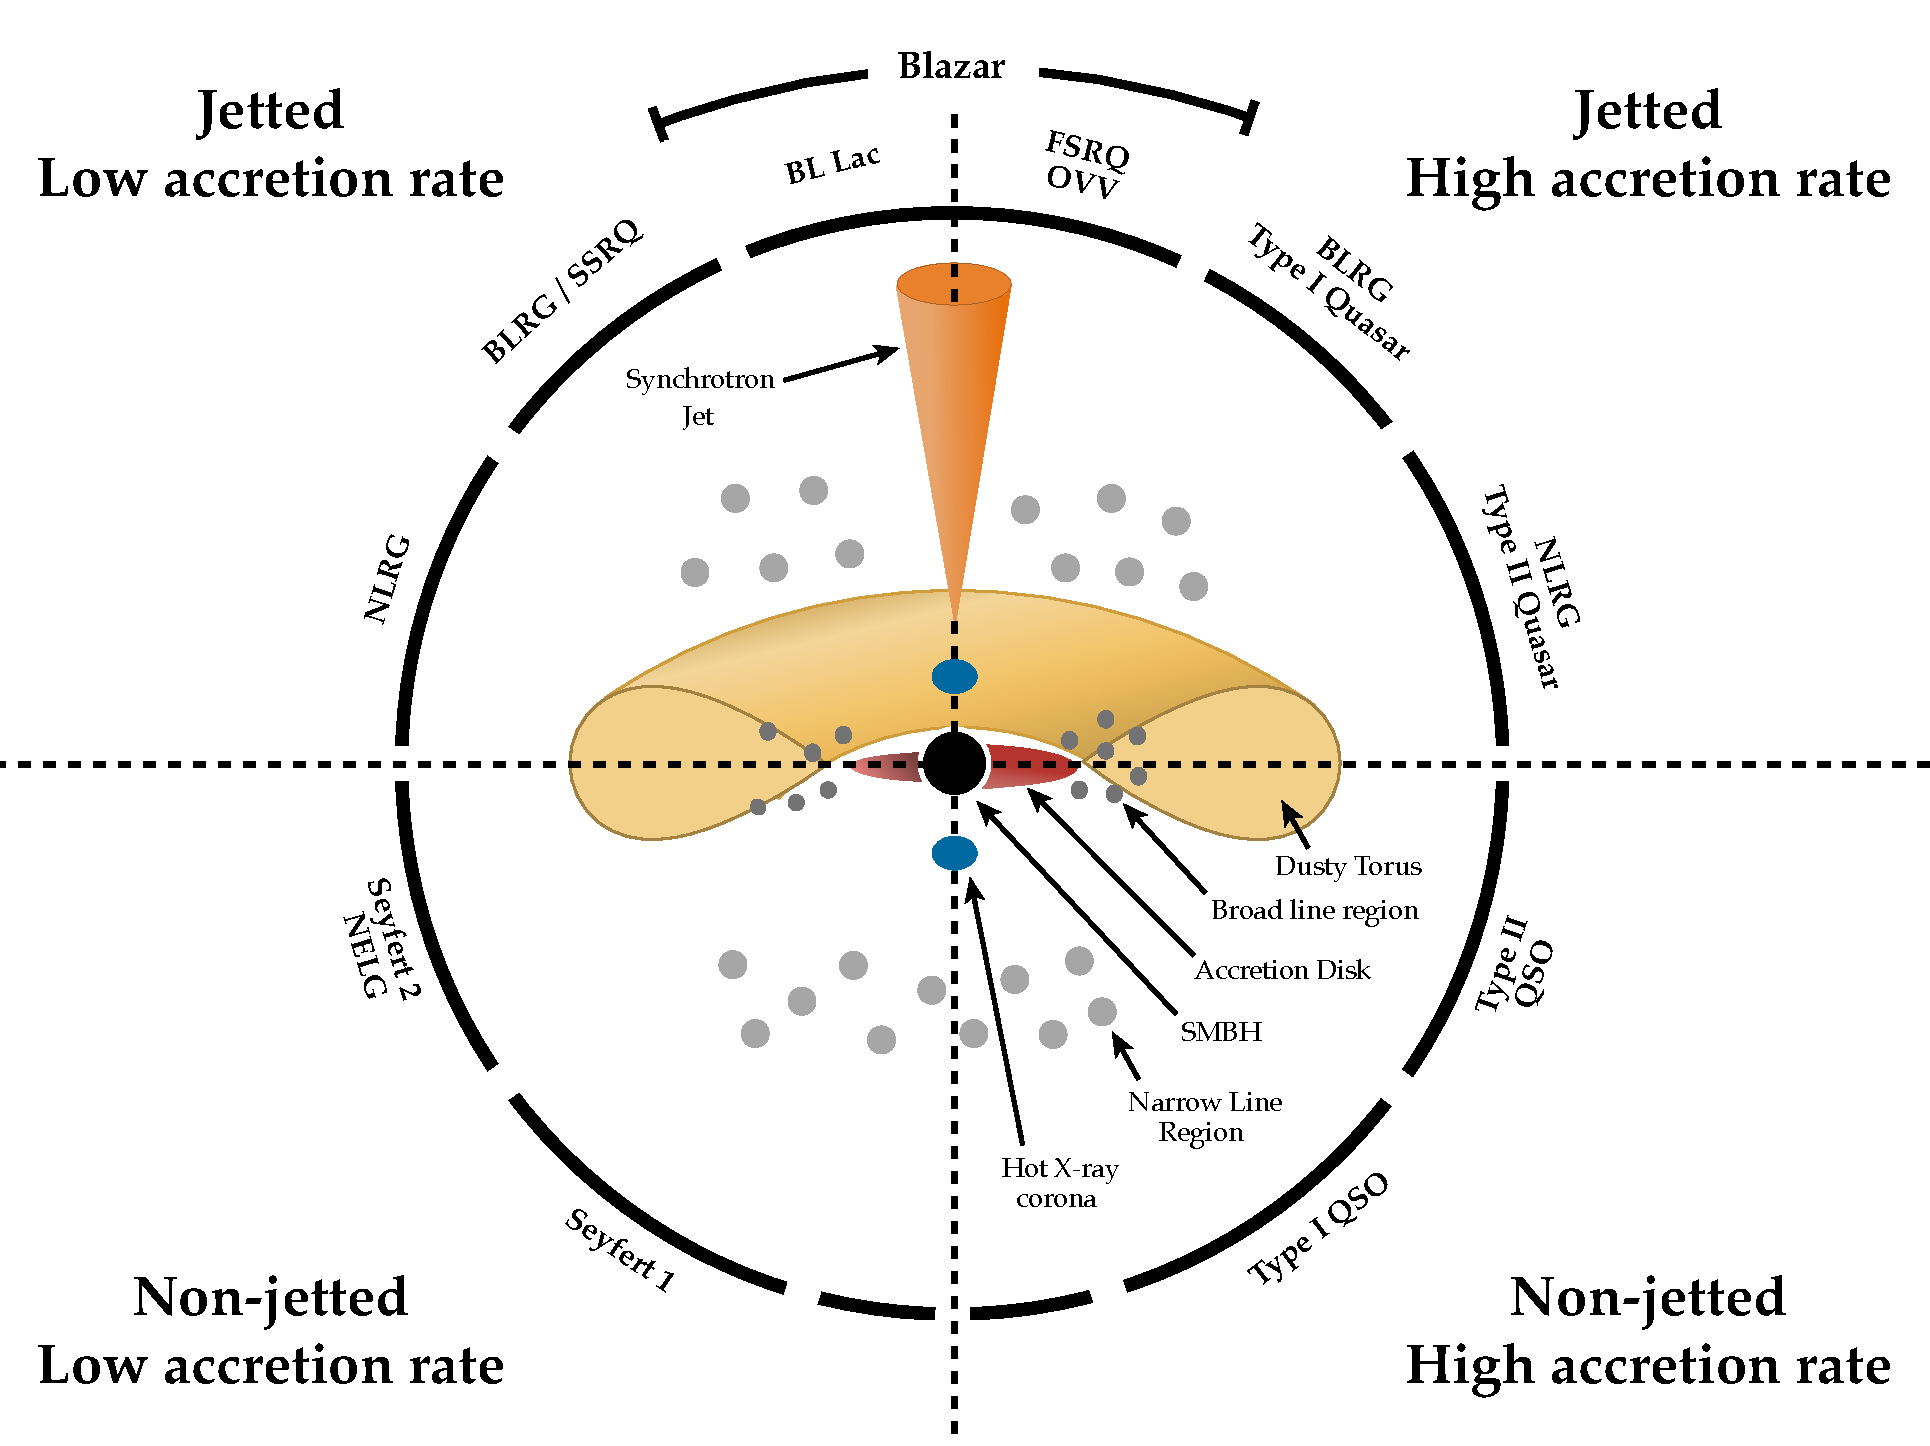
\includegraphics[width=0.7\textwidth]{theory/agn_unification.pdf}
    \caption[AGN]{AGN unification scheme. Depending on the viewing angle towards the AGN system, different source classes emerge. Following the argumentation of~\cite{Padovani2017}, the upper (lower) segment label radio loud (radio quiet) was changed to jetted (non-jetted). Adapted from~\cite{Thorne2022}.}
    \labfig{agn_unification}
\end{figure}

As can be seen in Fig.~\ref{fig:agn_unification}, these systems are thought to contain a SMBH in the center. The black hole is fed by a surrounding accretion disk of hot material, which in turn is enshrouded in a dusty torus.

\begin{marginfigure}
    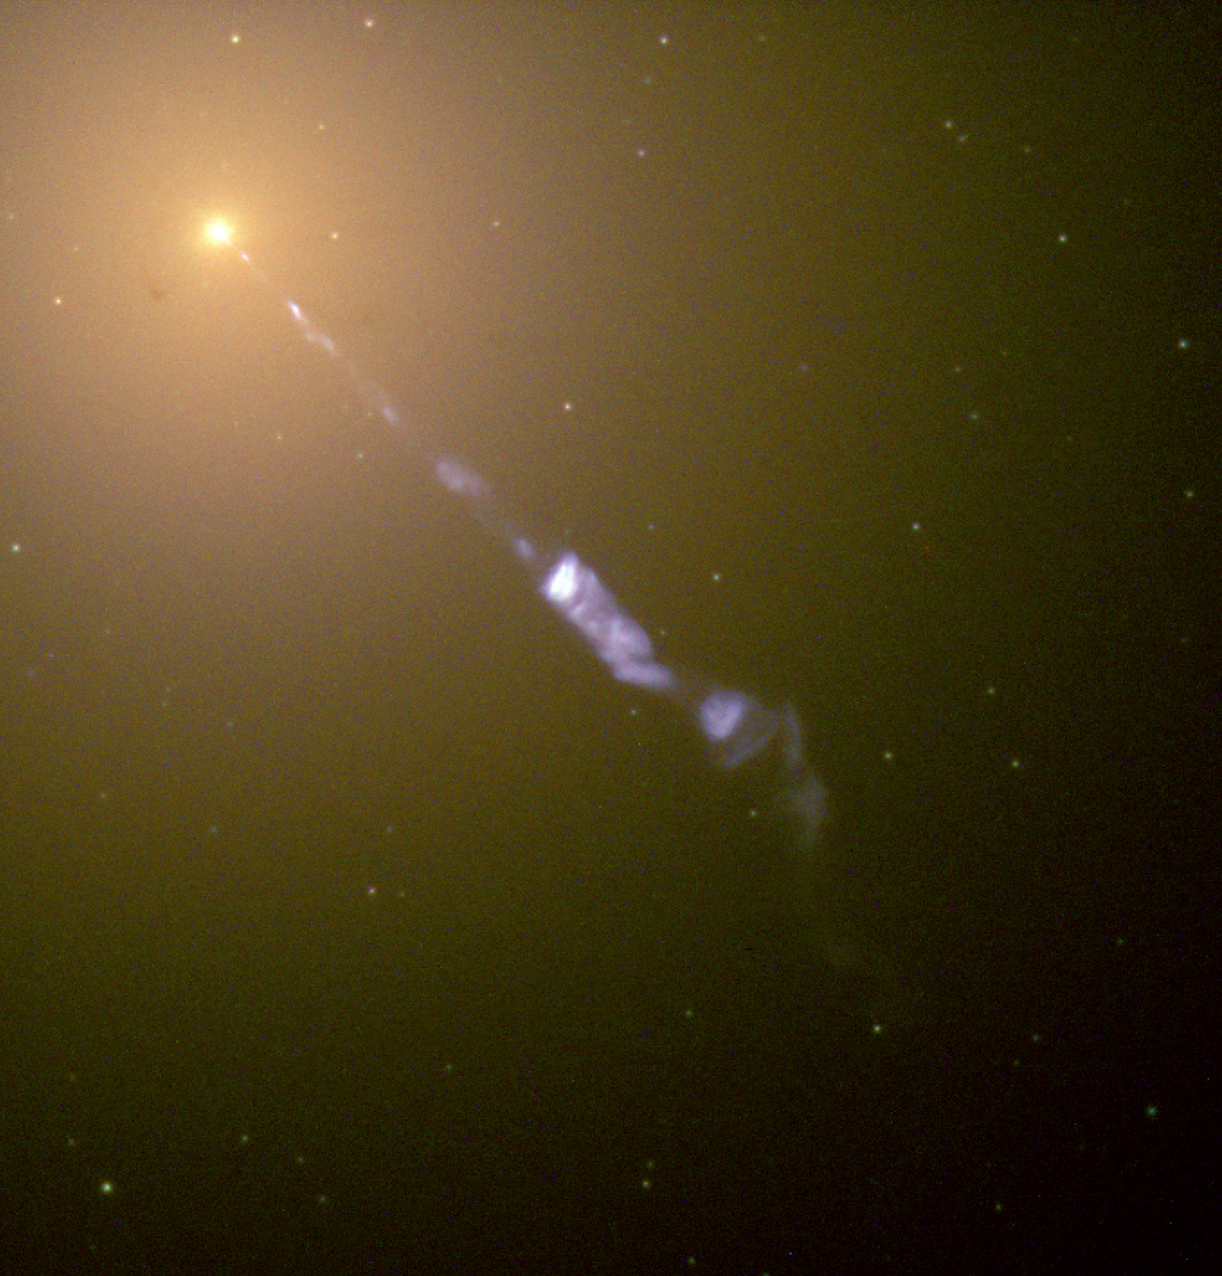
\includegraphics{theory/m87.jpg}
    \caption[M87 jet]{Hubble Space Telescope composite image of the jet launched by the AGN within M87, \SI{17}{\mega\parsec} away. Image credit: NASA/Hubble Heritage Team}
    \labfig{m87_jet}
\end{marginfigure}

Perpendicular to the accretion disk, often energetic jets of relativistic material are launched from the system. When one looks directly into the jet, the system appears as blazar (top of~\ref{fig:agn_unification}). If one moves away from the jet direction, the AGN will in general appear as Type I AGN, displaying broad emission lines stemming from the so-called Broad-Line Region (BLR), lying at a distance of \SIrange{e-2}{1}{\parsec} to the SMBH. It consists of gas clouds, and the Doppler-induced line-broadening suggests high velocities, resulting from the fact that the material is deep within the gravitational well of the SMBH.

Moving further away from the jet, one gradually moves into the Type II AGN class: The BLR close to the core gets hidden behind the dust torus, and only the  Narrow-Line Region (NLR) is still visible, as it is more distant from the core (\SIrange{e2}{e4}{\parsec}). Also here, gas heated by the core radiates, but the gas density is lower compared to the BLR, and from the line-broadening one can infer much lower velocities of \SI{\sim500}{\kilo\m\per\s}~\sidecite{Beckmann2012}.

If a jet is present, the AGN strongly emits in radio wavelengths. This is caused by the synchrotron emission of highly relativistic electrons. These AGN were labeled `radio loud', in contrast to `radio quiet' AGN without a jet.

AGN have been proposed as sources of high-energy neutrinos as early as the 1970s~\sidecite{Eichler1979}. The most promising site of high-energy neutrino production is the relativistic jet. In some cases such jets can be visually detected, like the prominent jet visible in M87 (see Fig~\ref{fig:m87_jet}). Jets are thought to be highly collimated, extremely energetic plasma structures launched from the accretion disk. Only a minority \SIrange{10}{20}{\percent} of observed AGN show evidence of such jets~\sidecite{Padovani2010}. Note that the intrinsic fraction of jetted AGN is considerably lower, with an estimate of \SIrange{0.1}{0.2}{\percent}.

When the electrons and protons contained in the jet plasma are clumped together in relativistically moving `blobs' and are spinning in magnetic fields, they emit synchrotron radiation~\sidecite{Combes2021}. This is the usual explanation for the first hump in a typical blazar spectral energy distribution (SED).

The explanation for the second hump is still debated. One scenario is that the synchrotron photons themselves form a target field for their `parent' electrons and protons. The former can interact with them via inverse Compton Scattering (CS), transferring energy to those photons. This process is called Synchrotron Self-Compton (SSC)~\cite{Spurio2018}, giving rise to the second hump. This was dubbed the Leptonic Model, and due to the absence of accelerated hadrons as e.g.\ protons, it does not predict the presence of high-energy neutrinos.

An alternative model to explain the second hump is the Hadronic Model. Here, the jet also contains a sizable fraction of hadrons~\sidecite{Reimer2012}. So not only the leptonic processes take place (Synchrotron radiation, inverse Compton scattering), but also the protons generate Synchrotron radiation. Additionally, the hadrons can interact with target photons in the vicinity, producing charged and neutral pions. These decay as detailed in Section~\ref{cr_interactions}, producing high-energy neutrinos in the process. Therefore, the detection of high-energy neutrinos from blazars is considered a smoking gun signature for hadronic acceleration processes~\sidecite{Gao2018}.

As the optical brightness of the AGN is driven by the synchrotron emission, it only traces the photon target field density for potential hadronic interactions, but not the proton luminosity itself.

\subsection{Tidal Disruption Events}

A Tidal Disruption Event (TDE) marks the end of a very unlucky star. When a star happens to approach the SMBH at the galactic center too closely, the resulting gravitation forces might overcome the star's self-gravity, tidally disrupting and destroying the star~\sidecite{Rees1988}. Roughly half the mass of the star is accreted around the black hole, and the bright electromagnetic flare created by this can shine for months. Nevertheless, the exact mechanisms at play causing this emission are still widely discussed~\sidecite{Gezari2021}.

TDEs have already been predicted in the 1970s~\sidecite{Hills1975}, and the first few TDEs were discovered in the 1990s and early 2000s in X-ray wavelengths. Optically detected TDEs arrived in the last decade~\sidecite{Velzen2011}, with steadily rising numbers in the last decade, mainly driven by optical all-sky survey telescopes like the Zwicky Transient Facility (ZTF, see Chapter~\ref{ztf}). Fig.~\ref{fig:tde_cumulative} shows the number of detected TDEs since 1995. As of December 2022, roughly 100 TDEs have been discovered in total, with more than 30 detected during the 2.6 years of ZTF Phase I alone~\sidecite{Hammerstein2022}.

TDEs normally emit a continuous spectrum that can be well approximated by a blackbody (see e.g.~\sidecite{Gezari2015} for a spectrum of \textit{PS1-10jh}, the prototypical Optical+UV TDE). Peculiarly, there seems to be a somewhat bimodal distribution of blackbody temperatures: One optical/UV population, and a second population peaking in the X-ray, better described by blackbodies of higher temperature~\cite{Gezari2021}.

As the accretion disk hypothesized  to form from the infalling material after the disruption will most likely be very hot, it is unclear what the cause of the optical/UV emission is. Furthermore, the blackbody radii inferred from the optical/UV emission exceed the size of the freshly formed accretion disk by $1-2$ orders of magnitude.

\begin{marginfigure}
    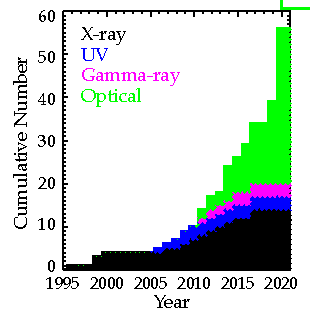
\includegraphics{theory/tde_cumulative.pdf}
    \caption[TDE detections]{Cumulative number of TDE detections, with the color encoding the discovery wavelength. The relative increase in the detection rate is driven by ZTF\@. Adopted from~\cite{Gezari2021}.}
    \labfig{tde_cumulative}
\end{marginfigure}

To date, multiple models have been brought forward to motivate the optical/UV emission, such as semi-relativistic outflows or winds, or diffusive shock acceleration stemming from the tidal stream intersecting itself~\cite{Gezari2021}.

If the material from the disrupted star is circularized rapidly, one interesting approach to unify the two populations (X-ray vs.\ optical/UV) is a viewing angle dependent model, akin to the unified AGN model presented in Section~\ref{agn}.

\begin{figure}[htb]
    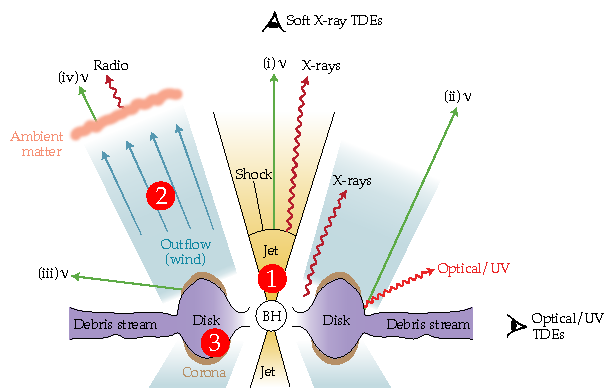
\includegraphics[width=0.9\textwidth]{theory/tde_unification.pdf}
    \caption[TDE Unification]{TDE unification model. The peak wavelength visible is a function of the viewing angle. Seen from above, the X-rays are dominating, while viewed edge-on, the TDE appears in the optical/UV\@. Adopted from~\cite{Hayasaki2021}.}
    \labfig{tde_unification}
\end{figure}

In this model, X-ray bright TDEs are those where one looks into the direction of a shock perpendicular to the accretion disk, or in the direction of an outflow. Optical/UV TDEs are systems viewed edge-on, where X-rays are obscured, and emission stems mainly from X-rays reprocessed in the outer disk or in outflow~\sidecite{Hayasaki2021}. Intermediate viewing angles will produce a mixture of both signals.

Also, about \SI{1}{\percent} of TDEs are expected to launch relativistic jets, like e.g.\ the recently discovered AT2022cmc~\sidecite{Andreoni2022}. Such jets (denoted as (1) in Fig.~\ref{fig:tde_unification}), as well as the possible winds/outflows (2) or a potentially present disk corona (3), have all been proposed as production sites of high-energy neutrinos, shown as green lines (see e.g.~\sidecite{Murase2020} for the non-jet production sites).

The timescales involved in the neutrino production are poorly constrained, as the systems are not very well understood yet. It is to be expected though that neutrino production would not predate the TDE and optical emission from the event.

\section{Established Counterparts and Limits}

\begin{figure}[htb]
    \centering
    \begin{subfigure}[b]{0.52\textwidth}
        \centering
        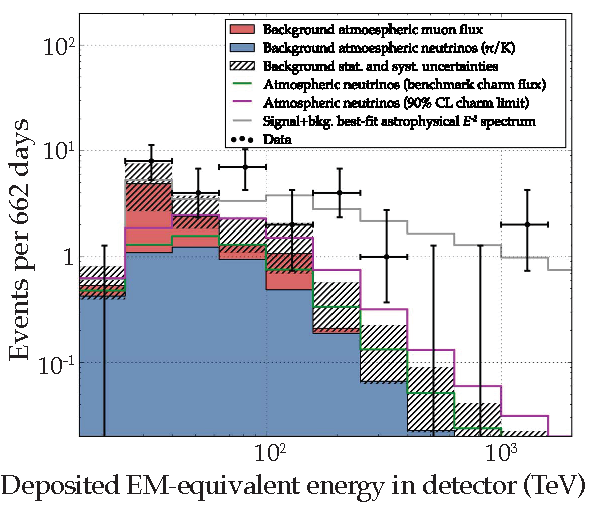
\includegraphics[width=1\textwidth]{theory/ic_first_spectrum.pdf}
    \end{subfigure}
    \begin{subfigure}[b]{0.47\textwidth}
        \centering
        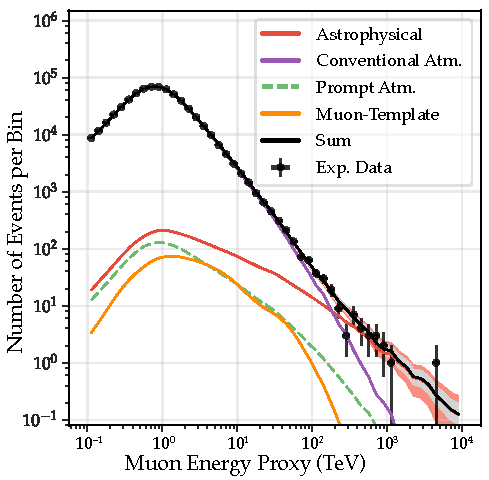
\includegraphics[width=1\textwidth]{theory/ic_last_spectrum.pdf}
    \end{subfigure}
    \caption[Astrophysical neutrino spectrum]{Left: Energy spectrum of the first astrophysical neutrinos, as detected by IceCube in 2013. The black points are the neutrinos measured, binned in energy deposited in the detector (a lower bound on the neutrino energy). The expected background rate of atmospheric muons (neutrinos) is shown in red (blue), and the gray line shows the best-fit astrophysical spectrum ($E^{-2}$ plus background.\ Right: Latest measurement of astrophysical neutrinos from a selection of track-like events (see Section~\ref{reconstruction}), including 9 years of IceCube data. Also here, the binned measurements are shown in black. Adapted from~\cite{Aartsen2013,Abbasi2022b}.}
    \labfig{ic_first_spectrum}
\end{figure}

In 2013, IceCube, a cubic-kilometer scale Cherenkov detector located within the Antarctic ice at the South Pole\sidenote{See Chapter~\ref{ic} for details} first detected two likely astrophysical \unit{\peta\eV} neutrinos at a significance of \SI{2.8}{\sigma}~\sidecite{Aartsen2013b}. Later that year, IceCube published more data, detecting high-energy astrophysical neutrinos at the \SI{4}{\sigma}-level~\sidecite{Aartsen2013}.

Fig.~\ref{fig:ic_first_spectrum} shows the first energy spectrum of high-energy neutrinos published by IceCube (left), as well as a more recent measurement from 9 years of IceCube data (right). At energies of roughly \SI{100}{\tera\eV}, the atmospheric background begins to recede, revealing a flux of astrophysical neutrinos that follows a power-law spectrum with a spectral index $\gamma\approx2.4$~\sidecite{Abbasi2022b}.

The flux is largely distributed isotropically over the sky, which stipulates an extra-galactic origin for the majority of high-energy neutrinos. The majority of this flux is still unaccounted for. Nevertheless, there are some prominent source candidates found since 2013. These, as well as upper limits on other hypothesized source populations, will be discussed next.

\subsection{AGN Counterparts and Limits}

\subsubsection{Blazar \emph{TXS 0506+056}}
In 2017, IceCube identified the blazar \emph{TXS 0506+056}, at the time flaring in gamma rays, as the probable source of high-energy neutrino \emph{IC170922A}~\sidecite{IC17922A,Aartsen2018}. The neutrino had an estimated energy of \SI{290}{\tera\eV}, and a best-fit sky location separated by \SI{0.1}{\degree} from the blazar, see left plot in Fig.~\ref{fig:txs}.

The blazar had a redshift of $z=0.337$~\sidecite{Paiano2018}, and a search for additional excess neutrinos from its sky location in 9.5 years of IceCube data found another episode of a \SI{3.5}{\sigma} excess of \num{\sim13.5} neutrinos between September 2014 and March 2015, stemming from the direction of \emph{TXS 0506+056}. However, during this period no significant gamma-ray flare was detected from \emph{TXS 0506+056}~\sidecite{Aartsen2018a}.

\begin{figure}[htb]
    \centering
    \begin{subfigure}[b]{0.47\textwidth}
        \centering
        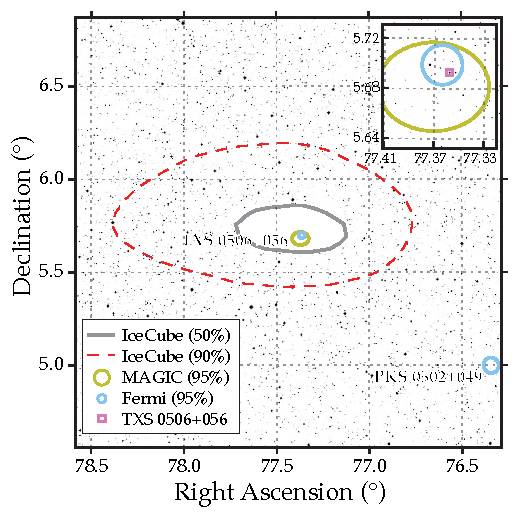
\includegraphics[width=1\textwidth]{theory/txs_localization.pdf}
    \end{subfigure}
    \begin{subfigure}[b]{0.52\textwidth}
        \centering
        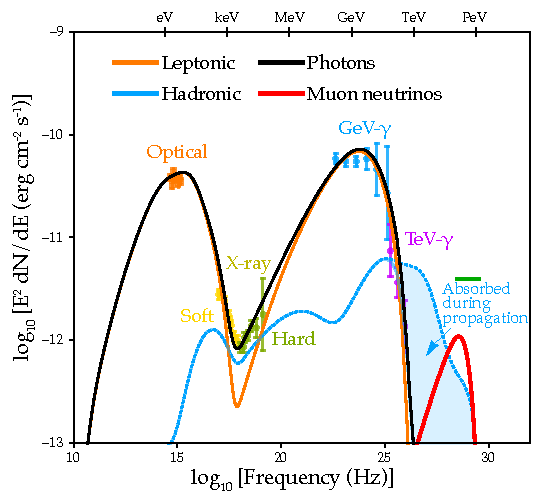
\includegraphics[width=1\textwidth]{theory/txs_modeling.pdf}
    \end{subfigure}
    \caption[TXS 0506+056: Localization and SED]{Left: Localization of the flaring blazar \emph{TXS 0506+056}, found in coincidence with high-energy neutrino \emph{IC170922A}. The \SI{50}{\percent} (\SI{90}{\percent}) localization contours of the neutrino location are shown in grey (dashed red).\ Right: Hybrid lepto-hadronic emission model to explain the SED, including the detected high-energy neutrino. The leptonic component is shown as orange line, while the hadronic component is shown in blue. The resulting combined photon spectrum is displayed in black, and the muon neutrino spectrum in red. Adopted from~\cite{Aartsen2018, Gao2018}.}
    \labfig{txs}
\end{figure}

The blazar (in its gamma-ray flaring state) has been shown to be able to produce a flux of high-energy neutrinos compatible with the IceCube detection~\sidecite{Gao2018}. An exemplary SED is shown in the right plot of Fig.~\ref{fig:txs}. Here, a `classical' hadronic scenario that would attribute the second hump entirely to decaying pions, was discarded to not overshoot the X-ray flux. Instead, the second hump was interpreted as a combination of leptonic and hadronic processes, with the former being the major contributor and the latter as strong as the X-ray bounds allow.

This lepto-hadronic model predicted a \SI{14}{\percent} probability of detecting a neutrino from the source without violating the bounds imposed by observations~\cite{Gao2018}. If one takes into account the large Eddington Bias~\sidecite{Strotjohann2019} expected for a single neutrino detection, this is still plausible. A consequence of this bias is that the neutrino flux of a single detection source could be systematically overestimated if that source is part of a large population emitting just below the IceCube detection limit, with occasional statistical overfluctuations.

However, producing the 2014--2015 neutrino flare without violating the gamma-ray limits proved to be a much harder challenge. No lepto-hadronic model\sidenote{to be consistent to the gamma-ray flaring state} able to produce more than 2--5 neutrino events during the time period could be found~\sidecite{Rodrigues2019} without violating the observational constraints. Reconciling the high number of neutrinos detected in the 2014--2015 period, without simultaneous gamma-ray flare, with the single neutrino from 2017, this time accompanied by a gamma-ray flare, remains a challenge.

\subsubsection{Type II AGN \emph{NGC 1068}}
The second AGN-neutrino association was \emph{NGC 1068}. This active galaxy is located relatively nearby, with a distance of \SI{\sim14}{\mega\parsec}~\sidecite{Abbasi2022}. It was classified as Type II AGN, i.e.\ an AGN without signs of a jet and viewed relatively edge-on, with dust obscuring the SMBH and the BLR (see Section~\ref{agn})~\sidecite{Rosas2022}. It has an exceptionally high rate of star formation~\sidecite{Eichmann2016}, and hosts outflows~\sidecite{Cecil1990}. Due to these features, it had already been proposed as a production site of high-energy neutrinos in the 1970s~\sidecite{Silberberg1979}.

In 2022, an archival study comprising IceCube data from 2011 to 2020 found an excess of $79^{+22}_{-20}$ neutrinos with \unit{\tera\eV} energies from the location of \emph{NGC 1068}. This results in a neutrino luminosity between 1.5 and \SI{15}{\tera\eV} of $L_\nu = (2.9 \pm 1.1_\text{stat}) \times \SI{e42}{\erg\per\s}$, exceeding the equivalent gamma-ray luminosity between 0.1 and \SI{100}{\giga\eV} by a factor of 18~\sidecite{Abbasi2022}.

NGC 1068 and TXS 0506+056 each contribute \SI{\sim1}{\percent} of the overall diffuse flux of astrophysical neutrinos measured by IceCube in their respective energy range. So far, it remains unclear if the diffuse flux is mainly composed of bright and nearby sources akin to \emph{NGC 1068}, a large population of faint sources with high redshifts ($z \geq 1$), or a mixture of both. Given the big difference in distance between \emph{NGC 1068} and \emph{TXS 0506+056} (the latter is about 100 times farther away) and the differences in their respective spectra, it seems plausible to assume at least two distinct AGN source populations~\cite{Abbasi2022}.

\subsubsection{Gamma-ray Blazar Limits}
However, there are several constraints on the contribution from AGN\@. A stacking analysis from 2019 investigated 1301 gamma-ray blazars from 3FHL~\sidecite{Ajello2017}, the third catalog of hard gamma-ray sources issued by the \textit{Fermi} Large Area Telescope (LAT)~\sidecite{Atwood2009}. After stacking and searching for spatial correlations between through-going high-energy muon tracks from the northern hemisphere, no excess of neutrinos was detected~\sidecite{Huber2019}. Assuming a spectral source index of $\gamma=2$, an upper limit on the contribution of blazars to the high-energy neutrino flux between \SI{119}{\tera\eV} and \SI{4.9}{\peta\eV} was found: Not more than \SI{17}{\percent} of the diffuse flux can be attributed to these sources~\sidecite{Huber2019}.

\subsubsection{MeV Blazar Limits}
The contribution of MeV blazars was also tested. 137 blazars from the \textit{Fermi} Low Energy Catalog (1FLE)~\sidecite{Principe2018}, detected below \SI{100}{\mega\eV}, were stacked. The result was compatible with a non detection. The upper limit derived from this---assuming a spectral index tracing the diffuse neutrino spectral index $\gamma=2.37$ and evaluated in an energy range between 30 and \SI{100}{\mega\eV}---was \SI{\sim1}{\percent} of the IceCube $\nu_\mu+\bar{\nu_\mu}$ flux~\sidecite{Abbasi_2022}.

\subsubsection{Jetted AGN Limits}

The correlation between high-energy alert neutrinos above \SI{200}{\tera\eV} with jetted (radio bright) AGN was also tested. The 3388 jetted AGN were selected from the Radio Fundamental Catalog\sidenote{\url{https://astrogeo.org/rfc}} by requiring X-band (\SIrange{8}{12}{\giga\Hz}) flux densities above 0.15 \unit{\jansky}. These were correlated with 56 published IceCube events with directional uncertainties below \SI{10}{\square\deg}. With these selections, a significant correlation was found, with a p-value of \SI{0.2}{\percent}~\sidecite{Plavin2020}.

However, a more recent study correlating this set of jetted AGN with the IceCube diffuse flux data comprising 10 years of muon tracks found no correlation~\sidecite{Abbasi2023a}. The unbinned maximum-likelihood-ratio method they employed gave no significant correlation between the neutrinos and the jetted AGN, resulting in an upper limit of an overall contribution to the \unit{\tera\eV}--\unit{\peta\eV} neutrino flux of \SI{30}{\percent}.

Furthermore, a recent study correlating blazars in the southern hemisphere (as the earth's core get opaque for neutrinos of the highest energies) from the Roma-BZCat Data Release 5 blazar catalog (5BZCat) with the 7 year all-sky map from IceCube found a correlation between blazars and high-energy neutrinos with a significance of $4.6~\sigma$. However, a follow-up study by IceCube was able to replicate the result, but when employing a 10-year neutrino all-sky map, the correlation vanished~\sidecite{Bellenghi2023}. This rather hints at a statistical fluctuation responsible for the 7-year map correlation.

\subsubsection{Non-jetted AGN Contribution}

The picture changes significantly when looking at non-jetted AGN: A recent study found a \SI{2.6}{\sigma} excess when correlating an infrared-selected subpopulation of non-jetted AGN with the astrophysical neutrino flux~\sidecite{Abbasi2022c}. The accretion disk luminosity of the AGN was estimated with the soft X-ray flux, and the source neutrino flux was weighted by that. The AGN population was selected based on their radio emission and infrared colors, and the \SI{2.6}{\sigma} excess (post trial) was obtained from the infrared-selected sample of 32249 AGN.

If this excess is interpreted as constituting a physical signal, it contributes $10^{+5}_{-4} ~\%$ of the diffuse flux at \SI{100}{\tera\eV}, see Fig.~\ref{fig:agn_ir_contrib}.

\begin{marginfigure}
    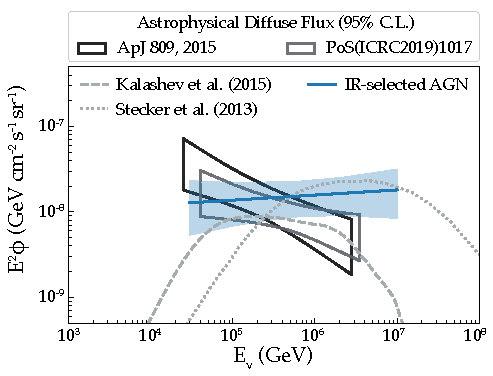
\includegraphics{theory/agn_ir.pdf}
    \caption[Non-jetted AGN]{Contribution of non-jetted AGN to the diffuse IceCube neutrino flux. The best-fit power law muon neutrino flux is shown in blue, corrected for completeness. Adapted from~\cite{Abbasi2022c}.}
    \labfig{agn_ir_contrib}
\end{marginfigure}

Correcting for completeness, \SIrange{27}{100}{\percent} of the observed \SI{100}{\tera\eV} neutrinos could stem from particle acceleration within the accretion disks or coronae of AGN~\cite{Abbasi2022c}.

\subsection{GRB Limits}
GRB limits can be drawn from a search for a correlation between 807 GRBs detected during a period of three years with IceCube high-energy neutrinos during that time. The search was constrained to prompt emission (see Section~\ref{grb}) from GRBs, excluding precursor events or GRB afterglows. This was achieved by looking for cascade events in the detector (see Section~\ref{reconstruction}), which are created by neutrinos of all flavor. These were required to be detected within the photon emission time as reported by the gamma-ray satellite one of 807 GRBs, the so-called prompt window. These prompt windows usually ranged from a few tens of seconds to a few minutes. This is highly favorable for coincident searches, as the tightly constrained window strongly suppresses background events. Six events were found to be time-correlated with neutrinos, but also consistent with background. If they are interpreted as genuine signal events, GRBs contribute less than \SI{1}{\percent} to the diffuse neutrino flux~\sidecite{Aartsen2016a}.

An additional search extended the time window considered in order to search for a correlation between a subset of GRBs contained in \texttt{GRBweb}\sidenote{\url{https://user-web.icecube.wisc.edu/~grbweb_public/}} and over 7 years of IceCube data. Also when using the expanded time window of \SI{e4}{s} sensitive to parts of the GRB afterglow, no time correlation could be found, with an upper limit on the contribution to the diffuse flux of \SI{24}{\percent}~\sidecite{grb_ul}.

\subsection{Supernova Limits}
This year, a study~\sidecite{Necker2023} was published correlating $1040$ core-collapse SNe with 7 years worth of IceCube neutrino events. The SN data was obtained from the Weizmann Interactive Supernova Data Repository \texttt{WiseREP}\sidenote{\url{https://wiserep.org/}}~\sidecite{Yaron2012} and the Open Supernova Catalog~\sidecite{Guillochon2017}.

The study looked at correlations between individual supernovae, as well as the stacked full sample. Both methods yielded results that are compatible with the null hypothesis. It assumed that the SN neutrino energy spectrum has a spectral index $\gamma=2.5$. Within the neutrino energy range of 1 to \SI{100}{\tera\eV}, the different types of SNe cannot contribute more than the following: SN IIP: \SI{59.9}{\percent}, SN IIn: \SI{33.9}{\percent} and stripped-envelope SNe (Ibc and IIb, see Section~\ref{sne}: \SI{14.6}{\percent} (assuming a choked-jet emission model)~\cite{Necker2023}.

The first two classes were tested with a set of emission time windows, ranging between 100 and 1000 days after the first detection, while the stripped-envelope SNe were tested for choked-jet emission, in which the neutrinos would predate the optical emission (see Section~\ref{grb}). In this case, the time window started 20 days prior to, and ending with the first optical detection.\ Neither SNe IIn and choked jet neutrino emission in stripped-envelope SNe can dominate the diffuse IceCube neutrino flux, while SNe IIP could still be dominant~\cite{Necker2023}.

\subsection{TDE Limits}
The last item to be discussed here is the limit from a stacking of TDEs. A search comprising 13 non-jetted and 3 jetted TDEs, correlating with 9.5 years of IceCube muon neutrino data, found no significant excess. Under the assumption of constant TDE neutrino luminosity, upper limits for their contribution to the diffuse were derived. These constrain jetted TDEs to less than \SI{\sim1}{\percent}, and non-jetted TDEs to less than \SI{26}{\percent} of the diffuse flux~\sidecite{Stein2019}.

\section{Conclusion}
The neutrino has been proposed, discovered and studied intensively. The detection of solar neutrinos, supernova neutrinos and finally the detection of a flux of high-energy neutrinos has firmly established the field of neutrino astronomy.

Nevertheless, the origin of the majority of the cosmic high-energy neutrino flux remains unclear. As can be seen in Fig.~\ref{fig:flux_ul}, no dominant source class has yet been established, though there are strong hints that non-jetted AGN contribute significantly to the diffuse neutrino flux. It is very much possible that the diffuse flux is composed of multiple source classes, each subdominant. The most stringent limits existing are those on prompt GRB emission and jetted TDEs, given their low rate density.

\begin{figure}[htb]
    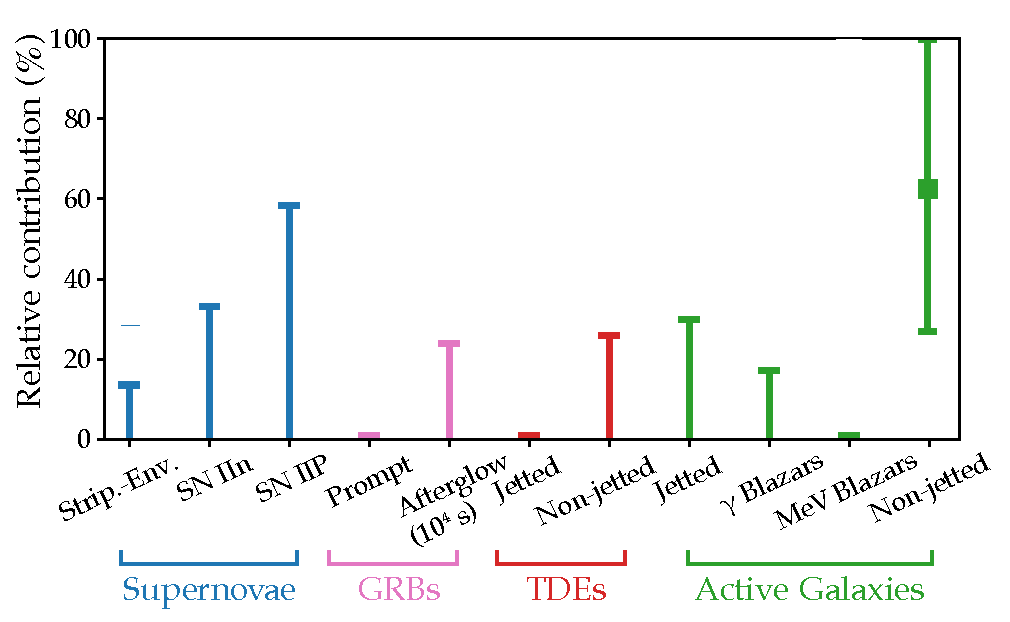
\includegraphics[width=1\textwidth]{theory/ul.pdf}
    \caption[Contribution to HE neutrino flux]{Potential source contributions to the diffuse IceCube high-energy neutrino flux. Adapted from a figure by Foteini Oikonomou from a talk at the \nth{27} European Cosmic Ray Symposium (ECRS), sent to the author in a private conversation. The values shown are mainly taken from~\cite{Guepin2022}, with some updates by the author. All numbers are discussed in the main text. Stripped-envelope SNe are denoted `Strip.-Env.' and a choked-jet emission model is assumed for these. Note that the unclear connection between the electromagnetic and expected neutrino flux, as well as uncertainties regarding the exact shape of the neutrino spectrum add significant uncertainties to these estimates.}
    \labfig{flux_ul}
\end{figure}

The absence of significant clustering of neutrinos, as well as little point sources in the data disfavors the hypothesis that rare and luminous objects are responsible for the majority of the flux~\sidecite{Guepin2022}. It is entirely possible that the bulk flux stems from numerous faint objects, which could render establishing a source class a challenging task.

\begin{marginfigure}
    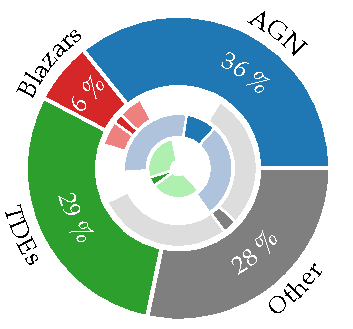
\includegraphics{theory/pie_chart.pdf}
    \caption[Neutrino flux contribution pie chart]{Pie chart of the contribution of known neutrino source classes as well as `other', comprising all source classes without association (main circle). The inner charts show the minimal (dark) and maximal (light) contribution within the \SI{90}{\percent} credible regions. Adapted from~\cite{Bartos2021} with minor error correction.}
    \labfig{pie_chart}
\end{marginfigure}

The flux could be fairly equally shared by AGN, TDEs and other sources, including blazars, as~\sidecite{Bartos2021} stipulate. The authors of the study estimated the contributions from source classes that have a known association (blazars: \emph{TXS 0506+056}, AGN: \emph{NGC 1068} and TDEs: \emph{AT2019dsg}\sidenote{The second neutrino associated TDE, \emph{AT2019fdr}, was not yet established.}) versus all other classes. They included statistical detection uncertainties, varying neutrino luminosity within source classes, as well as the redshift evolution of number density and properties of the individual source classes. The individual contributions are shown in Fig.~\ref{fig:pie_chart}, with the flux shared fairly equally between AGN, TDEs and other events, plus a noteworthy subdominant contribution by blazars.

Programs trying to establish a connection between individual high-energy neutrinos and sources within their localization are one good instrument in the available toolbox to solve the origin question at least partially. Such programs have the advantage of being time sensitive and allowing for follow-up observations necessary to classify ambiguous transients, contrary to archival studies. Chapter~\ref{fupipeline} will present one such program, a dedicated optical follow up to high-energy IceCube neutrinos.